\chapter{深度学习的可学习性}
\label{chap:deep-learning-theory}

设一个邮件分类神经网络已经把训练邮件全部分对。按前几章的经验，参数越多，模型越有余力去拟合训练邮件中偶然出现的细节，例如个别邮件的拼写错误或误标的标签；这些细节不会在新邮件中重现，所以训练错误率已经为零后再增加参数，新邮件上的错误率似乎应当上升。但实际中观察到的现象并不总是这样：训练错误率已经是零之后继续增加参数，新邮件上的错误率仍可能下降。要解释这一现象，我们需要分清两个问题：一是这个架构能不能把训练邮件分对，二是训练得到的神经网络能不能把尚未见过的邮件分对。“能把训练邮件分对”说明的是第一点，与第二点并不等价。本章关心的是，哪些架构、数据和训练条件能够同时支持这两种表现。

前面几章已经给出两类回答这种问题的工具。第一类看整个假设空间：VC维、Rademacher复杂度等量刻画空间有多灵活，再用一致收敛保证空间中每个函数的训练误差都接近新样本误差。第二类看具体算法：稳定性比较只替换一个训练样本时，算法输出改变多少；输出越不敏感，训练误差越能代表新样本误差。两类工具都还要配合“训练误差足够低”这一条件。

把这些工具用到神经网络，困难在于神经网络的假设空间通常极其灵活。第~\ref{sec:network-learning-problem}节将说明，同一个架构既能拟合真实标签，也能拟合与输入毫无关系的随机标签；只依赖架构本身的保证必须同时覆盖这两种情形，因而在实际样本量下给不出有用的数值。缺失的信息在于：训练最终从众多能拟合样本的参数中选中了哪一组，这一组有什么可度量的性质。本章据此依次考察训练结果的四个方面：参数的数值有多大，训练起点处的梯度给出了什么特征，更新路径偏向哪类解，以及能否把结果看作一族参数的分布。每条路线都先说明它补上前一条路线留下的哪个缺口，再通过复杂度或稳定性推导到期望风险，并同时交代训练误差和近似能力是否满足要求。

对于能直接分析的非线性神经网络，本章写明架构和范数条件；对于目前难以完整求解的训练过程，则先用线性回归、线性分类和深层线性神经网络看清机制，再说明结论可以推广到哪里。若模型规模、训练时长、任务或评价分布发生变化，学习问题本身也随之改变，需要按第~\ref{sec:learning-problem}节重新固定比较对象。

\section{神经网络的学习问题}
\label{sec:network-learning-problem}

\subsection{神经网络的架构与学习目标}

我们先固定待分析的预测函数。神经网络的参数是训练时调整的数值，通常包括连接系数和偏置；连接系数也称为权重，是参数的一部分，而不是参数的另一种名称。以下前馈神经网络省略偏置，因此每层的可学习参数就是连接系数，统一组成参数矩阵$\bm W_\ell$。激活函数和架构保持固定。每层先用参数矩阵组合输入，再逐坐标应用激活函数，末层作线性输出。ReLU激活$\phi(a)=\max\{0,a\}$保留正值、将负值置零，多层组合因而一般不再等价于一次线性变换。将包括线性输出层在内的变换层数记为$L$，神经网络为
\begin{equation}
 f_{\bm W}(\bm x)=\bm W_L\phi\bigl(\bm W_{L-1}\phi(\cdots\phi(\bm W_1\bm x)\cdots)\bigr),
 \label{eq:feedforward-network}
\end{equation}
其中$\bm W_\ell\in\mathbb R^{d_\ell\times d_{\ell-1}}$，$d_0$为输入维度，$d_1,\ldots,d_{L-1}$为隐藏宽度，$d_L$为输出维度，最大宽度为$w=\max_{0\leq\ell\leq L}d_\ell$。将各层参数矩阵的元素依次排成向量，得到$\bm\theta\in\mathbb R^p$，同一神经网络也记为$f_{\bm\theta}$。如果恢复偏置，还须把偏置分量计入$\bm\theta$和参数总数$p$。

举一个具体的尺寸。邮件用$d_0=1000$个词频特征表示，经过一个宽度$d_1=500$的隐藏层后输出一个分数，即$L=2$、$d_2=1$。两层参数矩阵分别是$500\times1000$和$1\times500$，共有$p=500{,}500$个参数。若训练集只有$n=10{,}000$封邮件，参数数是样本数的五十倍。$p$计量可调数值的个数，$L$计量依次变换的次数，两者都不是VC维；下一节会看到，VC维还取决于这些参数怎样组织成计算。卷五以隐藏层数计量神经网络层数；为便于对照外部结果，本章把隐藏层数记为$L_{\mathrm h}$，总变换层数为$L=L_{\mathrm h}+1$，上例中$L_{\mathrm h}=1$。引用外部结论时统一按总变换层数理解。

为了评价神经网络，取独立同分布样本$S=(z_1,\ldots,z_n)\sim\mathcal P^n$，$z_i=(\bm x_i,y_i)$。模型最终输出的预测记为$\widehat y=f_{\bm\theta}(\bm x)$，由“预测与真实标签是否吻合”定义的损失记为$\ell_{\mathrm{pred}}(\widehat y,y)$，例如分类的零一损失。把预测换成由参数$\bm\theta$和观测$z$确定，得到同一个损失的另一种写法$\ell_{\bm\theta}(z)=\ell_{\mathrm{pred}}(f_{\bm\theta}(\bm x),y)$；这只是把预测函数代入损失，并没有引入新的损失。这样记之后，就能直接使用第~\ref{sec:learning-problem}节的一般记号。样本平均与总体期望分别为
\[
 \hat R_S(\bm\theta)=\frac1n\sum_{i=1}^n\ell_{\bm\theta}(z_i),
 \qquad
 R_{\mathcal P}(\bm\theta)=\mathbb E_{z\sim\mathcal P}\ell_{\bm\theta}(z).
\]
算法利用经验风险选择参数，期望风险评价同一分布中新观测上的平均损失。分布明确时简写为$R(\bm\theta)$。讨论错误率时采用零一损失；推导梯度更新时损失须可微，届时另行写明平方损失或逻辑损失，避免把优化的目标和最终评价的错误率混为一谈。

如果某组参数使经验风险为零，就称模型能够\term{插值}（interpolation）这份样本，即在每个训练样本上都给出“完全正确”的预测。“完全正确”的含义随损失而变：平方损失要求预测数值逐项等于标签；零一损失只要求类别正确；交叉熵通常要在正确类别的分数趋于无穷时才趋于零，所以即使类别全部分对，交叉熵也仍大于零。\term{过参数化}（overparameterization）描述参数相对于样本数或拟合约束很充足的情形，常以$p>n$粗略表示，上面的邮件例子就是如此。参数多只是让插值成为可能；实际能否插值，仍取决于架构、数据和损失。

\subsection{VC维与样本量}

固定神经网络的架构后，我们要估计：为了使训练得到的分类器在新样本上接近这个架构能够达到的最低错误率，需要多少训练样本？可以先估计该架构所表示的假设空间的VC维，再利用前面的学习定理推导所需样本量。Baum与Haussler在1988年研究了神经网络规模与泛化样本数的关系，其分析涵盖阈值神经网络\scite{baum1988size}。这类样本量条件不要求输入和标签服从某一种特定的概率分布，所以称为分布无关的保证。不过，下面的保证以算法能够找到训练错误率最低的分类器为前提；它不说明梯度下降应怎样更新参数，也不保证梯度下降能够找到这样的分类器。

这里用容量描述一组分类器对不同标签安排的表达能力，具体采用VC维来衡量。考虑一组固定输入，任意给它们安排二分类标签；如果每一种安排都能由这个架构下的某组参数正确实现，就称该架构的假设空间能够打散这组输入。VC维是能够被打散的输入集合的最大大小，并不是假设空间中的函数总数。

用一个最简单的架构看这个定义。设输入是平面上的点，分类器是没有隐藏层的线性阈值单元$h(\bm x)=\mathbb I\{\bm w^\top\bm x+b>0\}$，用一条直线把平面分成两半。任取三个不共线的点，八种标签安排都能用一条直线分开，所以三点可以被打散。四个点则不行：若其中一点在另外三点构成的三角形内部，把内点单独标成一类就无法用一条直线分开；若四点构成凸四边形，按对角线交替标注两类同样无法分开。还要覆盖共线、点落在三角形边界等退化情形。对任意四个不同点$\bm x_i\in\mathbb R^2$，四个三维向量$(\bm x_i,1)$线性相关，故存在不全为零的$a_i$，使$\sum_i a_i\bm x_i=0$且$\sum_i a_i=0$。正系数与负系数分别归一化后，得到两组点的凸组合相等。把正系数组标成1、负系数组标成0，零系数对应的点任意标注；若能以严格正分数判1、非正分数判0，则同一个凸组合的分数在第一组必须为正，在第二组却非正，矛盾。因此任意四点都不能被打散，结合不共线三点的构造，平面线性分类器的VC维是3，而它恰好有3个参数$(w_1,w_2,b)$。这一巧合在神经网络中不再成立：有些架构的VC维远大于参数个数，也有些因结构受限而更小。

VC维说明架构能实现多灵活的分类，却不说明实际训练会得到哪个分类器。估计神经网络的VC维时，不仅要看参数个数，还要看连接方式、层数和激活函数。对分段线性神经网络，Bartlett等给出ReLU神经网络$O(pL\log p)$的VC维上界，并在相应参数范围内构造了达到$\Omega(pL\log(p/L))$的架构\scite{bartlett2019vc}。该下界只说明存在某些架构能够达到这样的VC维，不适用于每个含$p$个参数的架构。

有了架构对应的VC维上界，就能代入二分类学习基本定理。下面的定理采用前文的不可知PAC形式：它不假设架构中存在零错误的分类器，只要求算法输出的错误率接近架构内的最优错误率；$\varepsilon$是允许多出的错误率，$\delta$是允许保证失败的概率。下面把这一步统计推导单独写出，并保留“存在一个算法能达到该保证”与“实际优化算法能否找到对应参数”之间的区别：精确ERM具有相应统计保证，但这不保证梯度下降一定能找到经验风险最小的参数；若训练只实现近似ERM，还须计入后文说明的经验优化误差。

\begin{theorem}[有限VC维神经网络的不可知PAC样本量保证]
\label{thm:network-vc-pac}
设$(X,\mathcal X)$为可测输入空间，$Y=\{0,1\}$，
$Z=X\times Y$取乘积$\sigma$代数。固定神经网络架构所表示的非空二分类假设空间
$\mathcal H\subseteq Y^X$由可测函数组成，其VC维为有限数$d\geq1$。
对$Z$上的任意概率分布$\mathcal P$，令
$S=((x_1,y_1),\ldots,(x_n,y_n))\sim\mathcal P^n$，并定义零一损失下的
\[
 R_{\mathcal P}(h)=\mathbb P_{(x,y)\sim\mathcal P}\{h(x)\neq y\},
 \qquad
 \hat R_S(h)=\frac1n\sum_{i=1}^n\mathbb I\{h(x_i)\neq y_i\}.
\]
假设随机变量
$\sup_{h\in\mathcal H}|\hat R_S(h)-R_{\mathcal P}(h)|$可测。
存在通用常数$c>0$，使得任意$\varepsilon,\delta\in(0,1)$和任意
$\mathcal P$下，只要
\[
 n\geq c\frac{d\log(2/\varepsilon)+\log(2/\delta)}{\varepsilon^2},
\]
每个满足$\hat R_S(\hat h)=\inf_{h\in\mathcal H}\hat R_S(h)$的经验风险
最小化算法输出$\hat h$都以至少$1-\delta$的概率满足
\[
 R_{\mathcal P}(\hat h)\leq\inf_{h\in\mathcal H}R_{\mathcal P}(h)+\varepsilon.
\]
\end{theorem}
\begin{proof}
由有限VC维的一致收敛结论，在所给样本量下，可以使事件
$\sup_{h\in\mathcal H}|\hat R_S(h)-R_{\mathcal P}(h)|\leq\varepsilon/2$
以至少$1-\delta$的概率成立。在该事件上，对任意$h\in\mathcal H$有
\[
 R_{\mathcal P}(\hat h)
 \leq\hat R_S(\hat h)+\frac\varepsilon2
 \leq\hat R_S(h)+\frac\varepsilon2
 \leq R_{\mathcal P}(h)+\varepsilon.
\]
对右侧的$h$取下确界即可。证明使用了ERM的经验风险比较性质，没有给出实现ERM的
计算方法。
\end{proof}

因此，固定有限架构可以在所列前提下获得统计学习保证。证明的关键一步是：在高概率事件上，空间中每个分类器的训练错误率与新样本错误率相差都不超过$\varepsilon/2$，所以训练错误率最低的分类器在新样本上也不会比最优分类器差太多。

把数代进去，可以看出这条保证对大型神经网络意味着什么。忽略通用常数$c$，取$\varepsilon=0.1$、$\delta=0.05$，并设VC维$d=100$，右侧约为$(100\log 20+\log 40)/0.01\approx3\times10^4$。上一节的邮件神经网络有约$5\times10^5$个参数，按前面的上界，它的VC维可能达到参数数量级甚至更大，所需样本量就远远超出一万封邮件。更具体地，若把VC维粗略取为参数数$d\approx5\times10^5$，同样的$\varepsilon,\delta$下右侧约为$5\times10^5\times3.0/0.01\approx1.5\times10^8$，是手头样本数的一万五千倍；反过来，固定$n=10^4$，即使取$\varepsilon$接近1，右侧仍约为$5\times10^5\log2\approx3.5\times10^5$，所以在$(0,1)$中找不到满足条件的精度，这条保证对错误率没有任何约束。若手头样本数$n$未达到定理给出的充分样本量，这条定理就不能保证所要求的精度；这不等于更少样本一定无法学习，只说明这条按整个架构计算的保证派不上用场。另一类VC风险界对任意$n$都成立，却可能大于1而失去信息，不能把它当作上述样本量条件下的结论来用。实际训练若只实现近似ERM，还须计入经验优化误差。

\subsection{过参数化的挑战}

把训练标签换成随机标签，可以检验神经网络能否记住与输入无关的标注。Zhang等保持训练图像不变，把每张图像的类别标签独立替换为随机类别，再用相同架构和训练设置重新训练。在其部分实验中，神经网络仍能把训练图像全部分对\scite{zhang2021rethinking}。这里的“分对”只是复现人为指定的随机标签，并不表示识别出了图像的真实类别。由于这些随机标签与图像内容无关，记住它们并不能帮助预测新图像的真实类别。实验由此说明：神经网络能把训练数据拟合好，还不足以解释它为什么能预测新数据。

这个实验还说明，上一小节的数值困难并不只是常数取得不够精细。设图像有$K$个类别，随机标签与图像独立且均匀分布，那么任何分类器在这个“随机标签分布”下的期望错误率都是$1-1/K$；实验中训练出的分类器训练错误率却为零。于是在这份样本上，架构内至少有一个分类器的训练错误率与期望错误率相差$1-1/K$，$K=10$时为0.9。分布无关的一致收敛保证必须对随机标签分布同样成立，它在这一样本量下给出的差距上界就不可能小于约0.9。换句话说，只依赖架构和样本量的保证，无法区分“在真实标签上训练”与“在随机标签上训练”这两种情形，而这两种情形的期望风险恰恰相差悬殊。要解释真实标签下的泛化，必须引入能区分两者的信息：数据分布本身，以及训练在真实标签上实际得到的解有什么性质。

回到真实标签的学习问题，图~\ref{fig:learning-deep-selection}把架构、训练样本和算法的作用分开表示。架构确定可以选择哪些分类器；训练样本进一步筛出能把当前样本全部分对的分类器；算法最终得到其中一个。即使最后得到的分类器训练错误率为零，我们仍需分析它在新样本上的错误率。

\begin{figure*}[!htb]
  \centering
  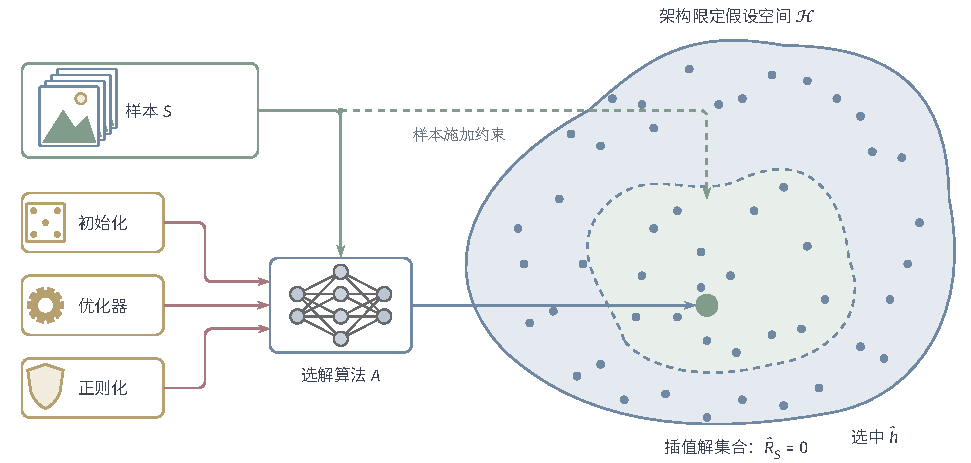
\includegraphics[width=164.600mm]{figures/03-foundations/02-learning-theory/tikz/learning-theory-deep-selection/figure.pdf}
  \caption{架构、样本和算法分别限定不同对象。外层是假设空间，内层是当前样本上经验风险
 为零的插值解集合；虚线表示样本施加的约束，实线表示算法的输入与输出。初始化、优化器
 和正则化参与选解。强调点仅示意算法选出一个插值解，不保证任意算法都实现插值；集合
 的形状和大小没有数值含义，插值也不保证期望风险小。}
 \label{fig:learning-deep-selection}
\end{figure*}

以训练邮件为例，能把它们全部分对的分类器，在新邮件上仍可能给出不同结果。一种做法仅记住这些训练邮件及其标签；另一种做法则根据邮件中的词语和链接等特征判断类别。两者都可能把当前训练邮件分对，但前一种做法没有告诉我们该怎样判断未见过的邮件。后一种做法只有在这些特征与类别的关系在新邮件中继续有效时，才可能保持较低的错误率。因此，增加能把训练样本分对的参数解，并不直接说明新样本上的错误率会降低。

即使样本和架构都固定，初始化、步长、优化器或正则化也可能让算法落到不同的插值解上，图中的算法箭头表示的就是这一步。于是，只知道插值解集合有多大还不够，我们还要知道算法从中选了哪一个。后面各节要回答两个问题：所选解具有什么可度量的性质，例如范数小、间隔大或对样本不敏感；训练为什么会偏向这样的解。

这种选解作用在模型规模变化时表现得尤为明显。设我们逐渐增加参数个数$p$，每次都把训练误差压到最低。参数少时模型拟合不了全部样本；当$p$大致增加到刚好能插值训练样本时（对线性回归而言约为$p\approx n$），称为到达\term{插值阈值}（interpolation threshold）。实验和理论都发现，某些模型的测试误差在这一阈值附近升高，继续增加参数后却重新下降，这种形态称为\term{双重下降}（double descent）\scite{belkin2019double}。图~\ref{fig:learning-double-descent}作定性示意。一种可能的机制是：在阈值附近，能插值的解几乎只有一个，它必须用很大的参数去拟合样本中的噪声，因而对噪声很敏感；越过阈值后，插值解多了起来，算法可以从中选到范数较小、对噪声不那么敏感的解。这一解释依赖数据和选解方式，并不保证增加参数总能降低风险。

图~\ref{fig:learning-double-descent}中的两条曲线评价不同对象。经验风险降到零附近，只说明拟合了当前样本；期望风险的峰值说明在该设定中新观测上的损失较高。要把峰值归因于对噪声敏感的解，还须另行比较相邻样本或噪声的影响。右侧风险下降说明增加参数后可能选到更合适的插值函数。这些差别都无法仅从训练风险判断。

欠定线性回归给出一个可以完全算清的选解例子。只有一个训练样本$\bm x=(1,1)^\top$、$y=1$时，参数$\bm w=(w_1,w_2)^\top$只需满足$w_1+w_2=1$，插值解是一整条直线。$(1,0)^\top$和$(1/2,1/2)^\top$都在这条直线上，但对新输入$(1,0)^\top$分别预测1和$1/2$。从零初始化做梯度下降，两个分量始终相等，最后只会停在$(1/2,1/2)^\top$，即直线上离原点最近的点。增加参数会改变这个最小范数解及其对噪声的响应，风险也可能随之改变。第~\ref{sec:implicit-bias}节将证明这一选解机制，并检查它的风险。

\begin{figure}[!htb]
  \centering
  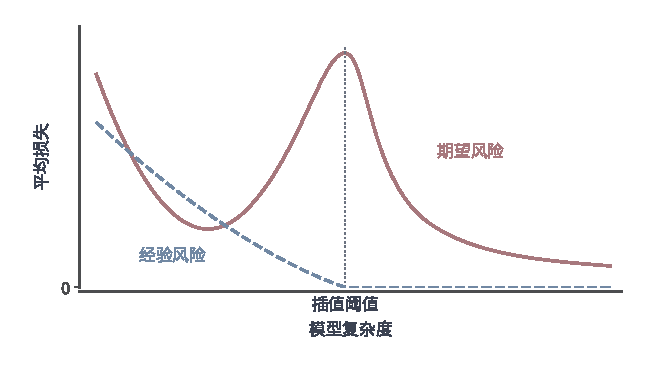
\includegraphics[width=112.000mm]{figures/03-foundations/02-learning-theory/matplotlib/learning-theory-double-descent/figure.pdf}
  \caption{双重下降的定性示意。虚线表示经验风险，实线表示一种可能出现的期望风险变化。
 插值后的期望风险还取决于算法如何选解。图中曲线用于说明概念，不是实验数据，
 也不表示所有神经网络都出现第二次下降。}
 \label{fig:learning-double-descent}
\end{figure}

由此可见，解释过参数化神经网络的泛化，关键是补充“算法选了哪个解、这个解有什么性质”的信息。下一小节先把这一问题写成统一的风险分解，再说明后面各节的分析路线分别从哪里补充这一信息。

\subsection{从一般学习理论到神经网络}
\label{sec:deep-general-learning}

为了让各路线回答同一个问题，我们把低训练损失与低总体损失之间的分析写成风险分解。算法$A$输出属于比较决策空间$\mathcal H$时，分别记期望泛化差与经验优化误差为
\[
 \begin{aligned}
 \Delta_n&=\mathbb E_S\bigl[R(A(S))-\hat R_S(A(S))\bigr],\\
 \rho_n&=\mathbb E_S\left[\hat R_S(A(S))-
                         \inf_{h\in\mathcal H}\hat R_S(h)\right].
 \end{aligned}
\]
相关期望存在时，有
\begin{equation}
 \mathbb E_S R(A(S))-\inf_{h\in\mathcal H}R(h)
 \leq\Delta_n+\rho_n.
 \label{eq:deep-risk-decomposition}
\end{equation}
推导只需在左边加减两个训练集上的量：
\[
 \begin{aligned}
 \mathbb E_S R(A(S))-\inf_{h}R(h)
 ={}&\Delta_n+\rho_n\\
 &+\Bigl(\mathbb E_S\inf_{h}\hat R_S(h)-\inf_{h}R(h)\Bigr).
 \end{aligned}
\]
最后一项不大于零：对任意固定的$h$，有$\inf_{h'}\hat R_S(h')\leq\hat R_S(h)$，两边对样本取期望并利用$\mathbb E_S\hat R_S(h)=R(h)$，得到$\mathbb E_S\inf_{h'}\hat R_S(h')\leq R(h)$，再对$h$取下确界即可。去掉这一项便得到此式。

式~\eqref{eq:deep-risk-decomposition}左边是算法输出函数的总体风险与$\mathcal H$内最优总体风险之差，也就是最终关心的超额风险；右边两项分别对应两个不同的缺口。第一项$\Delta_n$衡量算法所选函数在训练集上的平均损失，与它在新样本上的期望损失相差多少，即训练表现能否代表新样本表现；第二项$\rho_n$衡量算法所选函数在训练集上的损失，比训练集上的最优假设还差多少，即训练有没有把训练损失降到空间允许的最低水平。若这两项都小，就能保证算法输出在新样本上的总体风险接近$\mathcal H$内的最优风险。

用一组重复抽样的教学数值看两项各管什么。设$\mathcal H$内最低总体错误率为3\%。对同一样本量反复独立抽取训练集并运行同一算法，假设所选网络的平均训练错误率为1\%，训练集上最低错误率的平均值为0\%，所选网络的平均总体错误率为8\%。于是$\rho_n=1\%$、$\Delta_n=7\%$，右侧上界为8\%，实际的平均超额风险为$8\%-3\%=5\%$。这些数值都对训练样本的重抽样取了平均，不能由某一次训练的三个错误率直接得到。平均经验优化误差与平均泛化差分别占据上界的一部分；只减小前者，例如把平均训练错误率降到0，并不自动使平均总体错误率8\%下降，还须控制$\Delta_n$。

需要注意的是，$\Delta_n$评价的是根据训练样本选出的函数，而不是一个事先固定、与训练样本无关的函数。对固定函数，训练错误率是新样本错误率的无偏估计；但算法会挑选在这份样本上表现最好的函数，这一挑选本身就使训练错误率偏乐观。训练时，算法可能更多地拟合这份样本中特有的噪声，使训练损失下降，却没有使新样本上的期望损失同样下降，两种损失的差距就会扩大。因此，低训练损失仍需配合对$\Delta_n$的控制，才能支持低总体风险的结论。

一致收敛与稳定性是控制$\Delta_n$的两种办法，但比较对象不同。一致收敛对空间中所有假设同时估计经验风险与总体风险的差距，所以只要空间不太复杂，无论算法选了谁都有保证；稳定性只看实际算法，比较替换一个训练样本时输出改变多少。因此，架构不变时，初始化、正则化和优化方式不会改变架构的VC维，却可能改变算法的稳定性。

有了这两种控制$\Delta_n$的办法，后面四节分别从神经网络训练结果的一个方面出发，说明可以借哪种办法得到风险保证。四条路线各自在自己的条件下给出结论，不需要组合使用；同一个训练结果满足哪条路线的条件，就可以用哪条路线分析。它们的先后顺序按“前一条路线留下了什么问题”排列。

第~\ref{sec:network-norm-bounds}节针对的缺口是：VC维只数架构的参数和连接，看不到训练得到的参数取了什么数值。这条路线基于参数大小，只问训练结束时参数的范数有多大。范数限制了输入变化被放大的倍数，范数受限的神经网络无法任意细致地区分相近的输入，因而受限函数空间的复杂度较小，可以用一致收敛控制$\Delta_n$。结论对满足范数条件的所有神经网络同时成立，但它把“训练确实得到了范数小的参数”和“训练能把损失降下来”都当作前提，没有解释。

第~\ref{sec:neural-tangent-kernel}节补的正是训练这一环：非凸训练为什么能把损失降到零，降到零时选中了哪个函数。它基于初始化处的参数梯度，研究一种可以完整求解的情形：在特定的宽度和初始化缩放下，训练中参数只在初始化附近移动，神经网络近似等于以初始梯度为特征的线性模型，训练变成固定核上的核回归。这样既能算出训练会收敛到哪个函数，又能用核方法的复杂度或正则化稳定性给出风险。代价是依赖“特征几乎不变”这一近似，而实际神经网络的特征常在训练中明显改变。

第~\ref{sec:implicit-bias}节去掉“特征不变”这一近似，转而研究整条更新路径。插值解往往有无穷多个，梯度下降并不随机挑选，而是由初始化、损失和参数化共同决定偏向哪一类解，例如最小范数解或最大间隔方向。先证明训练选出的解具有这类结构，再用相应的复杂度界或稳定性得到风险。这条路线最贴近实际训练，但非线性神经网络的完整轨迹目前难以求解，完整证明只在线性回归、线性分类和深层线性模型等可解情形中得到。

第~\ref{sec:parameter-distributions}节换一个描述单位：既然逐个追踪参数点太难，就改为描述参数的分布。平均场方法把一个宽神经网络的大量神经元看作参数空间中的质量分布，它允许特征随训练改变，又不必追踪每个神经元；PAC--Bayes方法则把训练结果附近的一族神经网络看作随机预测器，用“这一族在扰动下仍然损失低”这一事实代替对单个参数点的最坏情形估计。两者都适用于参数点本身难以分析、但分布性质较易刻画的情形。

这四条路线都使用前面学习理论中的工具，并没有推翻那里的不可学习性结论。前面已证明：若零一损失分类面对任意的输入—标签联合分布，而假设空间的VC维无限，就不存在对所有分布都成立的PAC学习保证。这类不可学习性针对无限VC维空间，例如允许架构规模不受限制后形成的全类。固定有限架构即使VC维很大，也仍然有限；此时的困难是最坏情形样本量上界对实际样本量过于宽松，而不是已经证明该架构不可PAC学习。四条路线得到的保证都附带额外条件，例如参数范数受控、训练样本有足够的分类间隔、特征在训练中几乎不变，或训练算法对单个样本不敏感。这些条件排除了最坏情形的数据分布或最坏情形的训练输出（随机标签正是一种最坏情形：在随机标签上拟合所得的解通常不满足这些条件），所以风险界才能在样本有限时仍然有意义。它们回答的是“满足这些条件时风险有多大”，而不是为整个空间提供无条件保证。

比较各条路线的结论时，还要注意它们给出的保证在概率意义上并不相同。第一种是以高概率成立的风险界：对随机抽到的训练集，除了一个概率至多为$\delta$的坏情形外，所得模型的期望风险都不超过界的右边；它说的是“这一次训练大概率不会差”。第二种是对样本取平均的风险界：它控制的是$\mathbb E_S R(A(S))$，即把训练集反复重抽、多次训练后，期望风险的平均值；平均值小并不排除某一次训练结果很差，要得到高概率结论还须另外付出代价，例如用Markov不等式把平均界转成概率界，失败概率会随之变大。第三种是训练损失下降有多快：它是优化问题的结论，回答训练多少步后经验风险$\hat R_S$足够小，只控制风险分解中的$\rho_n$，完全不涉及新样本上的表现。三类结论回答的问题不同，不能用其中一类代替另一类；每条路线对训练算法提出的额外要求，也须在结论中一并保留。

\section{基于参数大小的可学习性}
\label{sec:network-norm-bounds}

上一节的随机标签论证表明，只看架构的保证无法区分拟合真实标签与拟合随机标签。我们要找一个由训练所得参数计算、并且在这两种情形下取值不同的量。最直接的候选是参数的数值大小：拟合与输入无关的标签，需要让神经网络对相近的输入给出截然不同的输出，这往往要求更大的参数。Bartlett等在图像分类实验中观察到，按下文谱复杂度归一化后的间隔，在随机标签上明显小于真实标签\scite{bartlett2017spectral}。这是经验观察，不是定理；本节要建立的，是“参数小、间隔大”在什么条件下能推出风险上界。

一种做法是事先限制参数向量或矩阵的范数，只对满足限制的神经网络估计风险。范数衡量参数数值的整体大小，而不是参数有多少个。考虑两个参数个数完全相同的单层分类器$\bm w^\top\bm x$：一个取$\bm w=(1,1)^\top$，另一个取$\bm w=(100,-99)^\top$。输入从$(1,1)^\top$变成$(1.01,1)^\top$时，前者的分数只改变0.01，后者却改变1。后者能用很小的输入差异区分样本，因而更容易拟合偶然的细节。参数范数正好记录这种放大能力，所以范数约束提供了参数计数没有利用的信息；在适当的输入尺度和分类间隔条件下，可以据此得到更有用的风险上界。不过，范数较小不等于只学到了有用特征，也不自动保证新样本上的错误率较低。

在多层神经网络中，这种放大由各层参数矩阵共同决定：输入的变化先被第一层放大，再被后续各层继续放大，所以分析时不能只把各层范数相加。本节先固定允许的范数范围，估计其中所有神经网络的训练损失与新样本期望损失之间的差距。下面依次说明分类问题为什么还需要间隔，再处理两层神经网络，最后处理多层的范数乘积。即使某个风险界不直接出现隐藏宽度，它仍依赖这些范数和间隔条件；训练算法能否得到满足条件的参数，则要由后面的算法分析另行回答。

\subsection{参数大小与分类间隔}

从线性预测看，Cauchy--Schwarz不等式给出$|\langle\bm w,\bm x-\bm x'\rangle|\leq\|\bm w\|_2\|\bm x-\bm x'\|_2$：输入改变$\|\bm x-\bm x'\|_2$，分数至多改变它的$\|\bm w\|_2$倍。上面两个分类器的范数约为$1.41$和$140.7$，正对应两者截然不同的敏感程度。神经网络的范数分析沿这一思路，考察全部参数共同形成的函数会把输入变化放大多少，而不只是数参数。Bartlett在1996年研究了适当条件下参数大小对泛化保证的作用\scite{bartlett1996weights}。

对于分类，只知道分数会变化多少还不够，还要知道分数离改判有多远。设有三个类别，真实类别为第一类。分数$(3,2,0)$与$(2.01,2,0)$都分类正确，但真实类别领先第二名的幅度分别为1和0.01。若每个分数都可能受到0.1的扰动，前者仍然正确，后者却可能被改判。我们将真实类别领先其余类别的幅度称为分类间隔。

\begin{definition}[分类间隔]
\label{def:network-margin}
设$f_{\bm W}:X\to\mathbb R^K$是分类分数函数。
其在带标签输入$(\bm x,y)$处的分类间隔定义为
\begin{equation}
 \operatorname{margin}_{\bm W}(\bm x,y)
 =f_{\bm W}(\bm x)_y-\max_{j\neq y}f_{\bm W}(\bm x)_j.
 \label{eq:network-margin}
\end{equation}
对于取值为$\{-1,+1\}$的二分类标签和标量分数$f(\bm x)$，定义间隔为$yf(\bm x)$。
\end{definition}

间隔为正时，真实类别分数高于其余类别。若各分数最多变化$\alpha$，真实类别分数最多降低$\alpha$，竞争类别分数最多升高$\alpha$，领先幅度最多缩小$2\alpha$；所以间隔大于$2\alpha$时仍保留正确分类。

范数和间隔必须一起评价。把所有分数同时乘以10，分类结果不变，间隔放大10倍，参数范数也放大10倍。若只看间隔，似乎模型变“稳”了；若只看范数，似乎模型变“复杂”了；两者的比值才不受这种整体缩放影响。下面的风险界正是通过范数与间隔之比来衡量复杂度。

\subsection{不显含宽度的期望风险界}

先看两层ReLU神经网络，写作$f(\bm x)=\sum_{j=1}^m a_j\phi(\bm w_j^\top\bm x)$，其中$\phi(u)=\max\{0,u\}$是ReLU。这个表达式可以按“一个隐藏单元做什么、输出层做什么”来读：第$j$个隐藏单元先用参数向量$\bm w_j$与输入做点积，再用ReLU把负值截断；输出层再用参数$a_j$对该单元的结果加权求和。增加隐藏宽度$m$，就是增加更多这样的单元。

宽度增加后，要让风险界不随之变大，关键是限制这些单元的总能力。隐藏单元能把输入放大多少，由$\|\bm w_j\|_2$控制；它在输出中占多大比重，由$|a_j|$控制。因此同时限制每个$\|\bm w_j\|_2\leq B$和$\sum_{j=1}^m|a_j|\leq A$后，无论单元数$m$是多少，所有单元加起来对输出的总放大都有上限。下面的函数类就是在这些约束下允许任意的隐藏单元数。得到的风险界不直接出现$m$，所以称为不显含宽度的界：固定范数约束、输入尺度和间隔尺度后，单纯加宽神经网络不会增大界中的附加误差项。

衡量这个函数类有多复杂，我们沿用定理~\ref{thm:rademacher-risk-bound}所用的经验Rademacher复杂度：给训练样本配上独立的随机正负号，看函数类中最能“迎合”这组随机符号的函数能达到多高的平均相关。函数类越能拟合任意符号，这个量越大，风险界中的复杂度项也越大。它直接依赖训练样本和函数类，而不经过参数计数，正适合这里“单元数任意、总范数受限”的函数类。由于零一损失不连续，证明中还要像第~\ref{sec:rademacher-complexity}节处理线性分类那样，用一个在间隔$\gamma$内线性过渡的间隔损失代替它，使Lipschitz收缩不等式可用；这正是间隔$\gamma$出现在界中的原因。

\begin{theorem}[两层神经网络的范数与期望风险]
\label{thm:two-layer-norm-risk}
设$n,d\geq1$，$X\subseteq\mathbb R^d$取Borel $\sigma$代数，
$Y=\{-1,+1\}$，$\mathcal P$为$X\times Y$上的概率分布，且
$S=((\bm x_1,y_1),\ldots,(\bm x_n,y_n))\sim\mathcal P^n$。
假设$\|\bm x\|_2\leq r$在$\mathcal P$下几乎处处成立。
在抽样前固定$A,B,r,\gamma>0$及$\delta\in(0,1)$，并令
\[
 \mathcal F_{A,B}=\left\{\bm x\mapsto\sum_{j=1}^m a_j\phi(\bm w_j^\top\bm x):
 m\in\mathbb N,\ \sum_{j=1}^m|a_j|\leq A,\ \|\bm w_j\|_2\leq B\right\},
\]
其中$\phi(a)=\max\{0,a\}$。则任意满足
$\|\bm x_i\|_2\leq r$的训练特征序列$(\bm x_i)_{i=1}^n$，该函数类的经验Rademacher复杂度满足
\[
 \widehat{\mathfrak R}_S(\mathcal F_{A,B})\leq\frac{2ABr}{\sqrt n}.
\]
对于样本$S$，以至少$1-\delta$的概率，所有$f\in\mathcal F_{A,B}$同时满足
\begin{equation}
 \mathbb P_{(\bm x,y)\sim\mathcal P}\{yf(\bm x)\leq0\}
 \leq\frac1n\sum_{i=1}^n\mathbb I\{y_i f(\bm x_i)\leq\gamma\}
 +\frac{4ABr}{\gamma\sqrt n}
 +3\sqrt{\frac{\log(2/\delta)}{2n}}.
 \label{eq:two-layer-margin-bound}
\end{equation}
这里把零间隔也计为错误，因此左侧同时控制采用任意固定平局规则时的零一损失期望风险。
\end{theorem}
\begin{proof}
固定独立随机符号$\sigma_i\in\{-1,+1\}$。$\sum_i\sigma_if(\bm x_i)=\sum_ja_j\sum_i\sigma_i\phi(\bm w_j^\top\bm x_i)$关于输出层参数是线性的；在$\sum_j|a_j|\leq A$的约束下，线性函数的最大值把全部权重$A$放在绝对值最大的那个单元上，并取与它同号的符号。所以输出层参数$\{a_j\}$的约束给出
\[
 \sup_{f\in\mathcal F_{A,B}}\sum_{i=1}^n\sigma_i f(\bm x_i)
 =A\sup_{\|\bm w\|_2\leq B}
 \left|\sum_{i=1}^n\sigma_i\phi(\bm w^\top\bm x_i)\right|.
\]
绝对值可分别用正号与负号的上确界之和控制；由于$\bm w=0$可取，这两个上确界都非负。
随机符号的对称性使它们的期望相同。再用ReLU的$1$-Lipschitz性质与收缩不等式，得到
\[
 \begin{aligned}
 \widehat{\mathfrak R}_S(\mathcal F_{A,B})
 &\leq\frac{2AB}{n}\mathbb E_{\bm\sigma}
       \left\|\sum_{i=1}^n\sigma_i\bm x_i\right\|_2\\
 &\leq\frac{2AB}{n}\sqrt{\sum_{i=1}^n\|\bm x_i\|_2^2}
 \leq\frac{2ABr}{\sqrt n}.
 \end{aligned}
\]
第二步使用Jensen不等式，交叉项因随机符号独立且均值为零而消失。

令斜坡损失$\psi_\gamma(u)$在$u\leq0$时为1，在$0<u<\gamma$时为$1-u/\gamma$，
在$u\geq\gamma$时为0。它上界零一错误指示函数，且为$1/\gamma$-Lipschitz。
固定样本标签后，$\sigma_i y_i$仍是独立随机符号，因此损失函数空间的经验Rademacher
复杂度不超过$\widehat{\mathfrak R}_S(\mathcal F_{A,B})/\gamma$。
应用定理~\ref{thm:rademacher-risk-bound}的经验复杂度形式，并用
$\psi_\gamma(y_i f(\bm x_i))\leq\mathbb I\{y_i f(\bm x_i)\leq\gamma\}$，
即得所述期望风险上界。
\end{proof}

定理右边有三项。第一项是训练样本中间隔不足$\gamma$的比例，比普通训练错误率更严格：分对了但领先不到$\gamma$的样本也计为失败。第二项是复杂度代价，由范数与间隔之比$AB r/\gamma$和样本量$n$决定。第三项是为了让结论以概率至少$1-\delta$成立付出的代价。

用一组教学数值读这个界。设输入已归一化为$r=1$，限制$A=B=1$，取间隔尺度$\gamma=0.5$，样本数$n=10{,}000$，$\delta=0.05$。复杂度项为$4\cdot1\cdot1\cdot1/(0.5\times100)=0.08$，置信项约为$3\sqrt{\log 40/20000}\approx0.041$。若训练后只有2\%的样本间隔不足0.5，则以至少95\%的概率，新样本错误率不超过$0.02+0.08+0.041\approx0.14$。这个结果与隐藏单元数$m$无关：$m$取100还是100万，只要$A,B$不变，界都相同。

隐藏宽度$m$没有直接出现在右侧，因此固定$A,B,r,\gamma$时，增宽神经网络不会提高充分样本门槛。但增宽若同时使训练出的$A,B$变大，或使更多样本的间隔变小，上界仍会变宽松。宽度之所以能从界中消失，正是因为这些量被事先固定。

也正因如此，用范数替代参数计数是一种有条件的分析。把ReLU神经网络的输出层参数整体乘以一个很小的正数，分类结果不变，范数与间隔却按同一比例缩小，式~\eqref{eq:two-layer-margin-bound}中的范数—间隔比并不改变。所以单靠压缩原始范数，不能对未加约束的分类空间给出PAC学习保证；该定理提供的是指定间隔尺度下的风险界。

我们可以把附加风险代价反解为样本门槛。给定$\varepsilon>0$，取
\begin{equation}
 n\geq\frac1{\varepsilon^2}
 \left(\frac{4ABr}{\gamma}
       +3\sqrt{\frac{\log(2/\delta)}2}\right)^2,
 \label{eq:two-layer-sample-requirement}
\end{equation}
就使式~\eqref{eq:two-layer-margin-bound}在经验间隔错误率之外的两项不超过$\varepsilon$。若训练输出有至多$a$比例样本未达到$\gamma$间隔，则以概率至少$1-\delta$，零一风险不超过$a+\varepsilon$。门槛控制样本评价到总体评价的附加代价，$a$能否降低仍取决于训练与数据。

减小范数与增大正确间隔都可改善这个上界，但单独压缩参数可能让更多样本达不到间隔$\gamma$，使第一项变大，两者之间存在取舍。范数—间隔比固定时，样本量增为四倍，附加误差界减半；在上面的例子中，$n$从一万增到四万，复杂度项从0.08降到0.04。这是充分界的缩放，既不保证实际测试错误减半，也不证明更少样本不能学习。

\subsection{深层神经网络的谱复杂度}

两层的分析依赖输出层参数之和这一特殊结构，深层神经网络无法直接沿用。这里要先回答一个更基本的问题：输入的一个小扰动穿过多层后，会被放大多少？衡量单层放大倍数的量是谱范数$\|\bm W\|_2$，它是单位向量经矩阵变换后可能达到的最大长度，也等于最大奇异值。例如$\bm W=\operatorname{diag}(3,0.5)$把第一个坐标方向拉长3倍，把第二个方向压缩一半，所以$\|\bm W\|_2=3$。扰动逐层传递时，每层至多放大$\|\bm W_\ell\|_2$倍，激活为$a_\ell$-Lipschitz时再至多放大$a_\ell$倍，所以总放大倍数不超过各层因子的乘积。三层谱范数都是2的神经网络，总放大至多为$2^3=8$。图~\ref{fig:learning-spectral-product}沿同一输入变化展示这些乘积。后面采用ReLU等1-Lipschitz激活，故激活因子为1。

\begin{figure}[!htb]
  \centering
  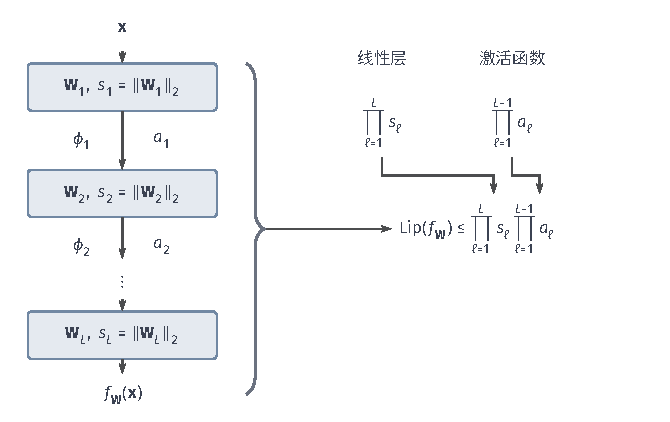
\includegraphics[width=112.000mm]{figures/03-foundations/02-learning-theory/tikz/learning-theory-spectral-product/figure.pdf}
  \caption{谱范数与激活函数共同控制输入扰动。第$\ell$层线性变换至多放大$s_\ell=\|\bm W_\ell\|_2$倍，层间激活再至多放大$a_\ell$倍；末层为线性输出。右上方两类因子分别连到乘积上界，大括号归并各层作用。当激活均为$1$-Lipschitz时，只剩谱范数乘积；该乘积仍不是完整的泛化复杂度。}
 \label{fig:learning-spectral-product}
\end{figure}

放大倍数受控还不等于函数空间简单。谱范数不超过2的矩阵仍有无穷多个，它们指向不同方向，组合出的函数也各不相同。我们还需要估计这些函数“实际有多少种”。常用的办法是统计覆盖数：在给定精度下，至少需要多少个代表函数，才能使空间中每个函数都离某个代表足够近（可参考\BookVolumeRef{vol:mathematical-preliminaries-upper}{卷1《数学准备：计算、分析与几何》}）。代表越少，空间越简单，风险界中的复杂度项也越小。

谱范数只记录一层在最强方向上的放大倍数，却看不出这一层“同时用了多少方向”。两个谱范数都为1的矩阵，一个只有一行非零，只能沿一个方向读取输入；另一个是单位矩阵，可以在所有方向上分别读取。在输入有界时，前者给出的输出只是一个一维投影的函数，后者保留了输入的全部方向，后续各层能据此组合出更多不同的函数，覆盖时也需要更多代表。为了把这一差别计入覆盖数，Bartlett等还用到行分组范数，即矩阵各行向量长度之和：$\|\bm A\|_{2,1}=\sum_i\|\bm A_{i,:}\|_2$。由于每一行的长度都不超过谱范数，而各行长度之和又不小于谱范数，比值$\|\bm A\|_{2,1}/\|\bm A\|_2$总在1与非零行数之间。对$100\times100$单位矩阵，100个方向各占一份，比值为100；只有一行非零时，比值恰为1。这个比值比较各行长度之和与整层最大放大倍数，既受行大小影响，也受各行的方向关系影响；它不是奇异方向数或矩阵秩。同为秩1，只有一行非零时比值为1，而$m$个相同行时比值为$\sqrt m$。在下面其他范数约束保持一致的界中，较小的行分组比值会减小覆盖数代价，但不能单凭它断言所有函数只沿少数奇异方向变化。对无偏置、1-Lipschitz且零点为零的激活神经网络，Bartlett、Foster与Telgarsky给出了衡量函数相对零函数规模的复杂度量（对应文献中取参考矩阵为零的情形）：
\begin{equation}
 \mathcal C(\bm W)=
 \left(\prod_{\ell=1}^L\|\bm W_\ell\|_2\right)
 \left[\sum_{\ell=1}^L
 \left(\frac{\|\bm W_\ell\|_{2,1}}{\|\bm W_\ell\|_2}\right)^{2/3}
 \right]^{3/2}.
 \label{eq:spectral-margin-bound}
\end{equation}
其中乘积项控制扰动在层间传播时的放大，求和项则进入覆盖数的估计。例如三层的谱范数都为2、上述比值都为4时，$\mathcal C=8\times(3\times4^{2/3})^{3/2}\approx166$；若把每层比值降到1，复杂度降为$8\times3^{3/2}\approx42$。复杂度量随层数、各层放大倍数和方向分布变化，却不直接数参数。这里按各谱范数非零书写，零矩阵层另行处理。下面采用事先固定范数上限的版本，用这个复杂度量推出样本量与风险界\scite{bartlett2017spectral}。

\begin{theorem}[深层神经网络的谱复杂度与期望风险]
\label{thm:spectral-network-risk}
设$n,L\geq1$，固定维数$d_0,\ldots,d_L\leq w$且$d_L\geq2$，输入空间
$X\subseteq\mathbb R^{d_0}$取Borel $\sigma$代数，标签空间
$Y=\{1,\ldots,d_L\}$。对
$\bm W_\ell\in\mathbb R^{d_\ell\times d_{\ell-1}}$，定义无偏置神经网络
\[
\begin{aligned}
 \bm h_0(\bm x)&=\bm x,\\
 \bm h_\ell(\bm x)
 &=\phi_\ell(\bm W_\ell\bm h_{\ell-1}(\bm x)),
 \qquad 1\leq\ell<L,\\
 f_{\bm W}(\bm x)&=\bm W_L\bm h_{L-1}(\bm x).
\end{aligned}
\]
其中各$\phi_\ell$固定、逐坐标作用、为$1$-Lipschitz且在零点为零。定义
\[
 \operatorname{margin}_{\bm W}(\bm x,y)
 =f_{\bm W}(\bm x)_y-\max_{j\neq y}f_{\bm W}(\bm x)_j.
\]
对任意矩阵$\bm A$，记
$\|\bm A\|_{2,1}=\sum_i\|\bm A_{i,:}\|_2$。
设$\mathcal P$为$X\times Y$上的概率分布，
$S=((\bm x_1,y_1),\ldots,(\bm x_n,y_n))\sim\mathcal P^n$，并令
\[
 R^{01}(\bm W)
 =\mathbb P_{(\bm x,y)\sim\mathcal P}
   \{\text{固定平局规则下 }f_{\bm W}\text{ 的预测不等于 }y\}.
\]
在抽样前固定$r,\gamma,s_\ell,b_\ell>0$及$\delta\in(0,1)$，并令
\[
 \mathcal C_0=
 \left(\prod_{\ell=1}^L s_\ell\right)
 \left[\sum_{\ell=1}^L(b_\ell/s_\ell)^{2/3}\right]^{3/2}.
\]
若$\|\bm x\|_2\leq r$在$\mathcal P$下几乎处处成立且$n\geq2$，
则以至少$1-\delta$的概率，
所有满足$\|\bm W_\ell\|_2\leq s_\ell$、
$\|\bm W_\ell\|_{2,1}\leq b_\ell$的神经网络同时有
\begin{equation}
 \begin{aligned}
 R^{01}(\bm W)\leq{}&\hat R_{S,\gamma}(\bm W)+\frac8n\\
 &+\frac{72r\mathcal C_0\log(2w)\log n}{\gamma\sqrt n}
 +3\sqrt{\frac{\log(1/\delta)}{2n}},
 \end{aligned}
 \label{eq:spectral-risk-explicit}
\end{equation}
其中
$\hat R_{S,\gamma}=n^{-1}\sum_i
\mathbb I\{\operatorname{margin}_{\bm W}(\bm x_i,y_i)\leq\gamma\}$
为经验间隔错误率，预测使用固定的平局规则。
\end{theorem}
\begin{proof}
采用Bartlett等论文附录引理A.8的固定范数约束界。
该引理的复杂度项为
$72\|\bm X\|_F\mathcal C_0\log(2w)\log n/(\gamma n)$，
其中$\bm X$的各行为训练样本中的特征向量。由$\|\bm x_i\|_2\leq r$可得
$\|\bm X\|_F\leq r\sqrt n$，代入便得到所述形式。
这里使用了外部引理中的神经网络覆盖数估计，不把该组合估计视为已在本章证明。
\end{proof}

上界在经验间隔错误率外保留三项余量。指定附加误差$\varepsilon>0$后，选$n$使
\[
 \frac8n+\frac{72r\mathcal C_0\log(2w)\log n}{\gamma\sqrt n}
 +3\sqrt{\frac{\log(1/\delta)}{2n}}\leq\varepsilon,
\]
即可得到概率至少$1-\delta$的$R^{01}(\bm W)\leq\hat R_{S,\gamma}(\bm W)+\varepsilon$。这是一条可逐个试代$n$的充分条件；忽略对数因子，门槛为$\bigl((r\mathcal C_0/\gamma)^2+\log(1/\delta)\bigr)/\varepsilon^2$量级。深度和宽度仍通过$\mathcal C_0$及对数参与，因此只替代了粗略参数计数，没有消除结构影响。

固定输入尺度、间隔尺度，并比较经验间隔错误率相近的神经网络，较小谱复杂度给出较小风险上界。复杂度项主导且忽略对数变化时，$\mathcal C_0/\gamma$减半可将同一附加误差的充分样本量约降为四分之一。然而，上界较小不证明实际错误率较低；上界大于1时尚不能提供非平凡分类保证。用一组教学数值看后一点：取$r=1$、$\mathcal C_0/\gamma=100$、宽度$w=500$、$n=10^4$，复杂度项约为$72\times100\times\log1000\times\log10^4/100\approx72\times6.9\times9.2\approx4.6\times10^3$，远大于1。这类常数和对数因子使界在常见规模下往往没有数值意义；它更可靠的用途是揭示风险依赖哪些量，以及在其他条件相同时比较不同训练结果。经验间隔分布与复杂度需要共同观察。

范数上限与间隔尺度在这条定理中必须先于样本固定。原因是：如果先看训练结果再挑选上限，就相当于从许多候选上限中挑出最有利的一个，挑选本身也会使界偏乐观。若训练后再选择它们，应事先列出一串候选上限（例如$1,2,4,8,\ldots$），对它们同时建立保证，并把失败概率$\delta$分摊到各候选上，代价是多出一个对数项；文献中的自适应版本做的正是这件事。不能直接把事后测量值代入固定约束而遗漏选择代价。

ReLU对正数缩放保持线性，即具有正齐次性（$c>0$时$\phi(cu)=c\phi(u)$）。因此把第一层参数乘以$c$、第二层参数除以$c$，神经网络表示的仍是同一个函数。例如取$c=10$，第一层谱范数放大10倍、第二层缩小10倍，乘积不变；每层的比值$\|\bm W_\ell\|_{2,1}/\|\bm W_\ell\|_2$也不受整体缩放影响。所以$\mathcal C$不会把这两种等价表示误判为不同的分类能力。若改用各层范数之和，这个和却会从$s_1+s_2$变为$10s_1+s_2/10$，对同一函数给出不同复杂度。

\term{Schatten范数}（Schatten norm）按奇异值的$p$范数（$1\leq p\leq\infty$）汇总矩阵的谱规模；非零矩阵的稳定秩则用总平方谱能量除以最大奇异值平方，零矩阵另约定为零。这些量与依赖坐标的行分组量不同（可参考\BookVolumeRef{vol:mathematical-preliminaries-upper}{卷1《数学准备：计算、分析与几何》}）。不同风险界使用不同谱量，式~\eqref{eq:spectral-margin-bound}采用的是行分组比值，不能直接换成稳定秩。

同一套逐层放大的计算还可以用于稳定性路线。前面比较的是同一函数空间中的所有神经网络；现在改为比较两份只差一个样本的训练集分别训练出的两个神经网络。若第$\ell$层参数因替换样本至多改变$\alpha_{\ell,n}$，这一改变会经后续各层继续放大后到达输出。因此下面的定理同时需要两类量：各层范数上限$s_j$控制放大，参数变化$\alpha_{\ell,n}$控制起点处的扰动。

\begin{theorem}[分层参数稳定性与期望泛化差]
\label{thm:layerwise-parameter-stability}
设$n,L\geq1$，$(X,\mathcal X)$为$\mathbb R^{d_0}$的可测子空间，
$(Y,\mathcal Y)$为标签空间，$\mathcal P$为$X\times Y$上的概率分布，且
$S=((\bm x_1,y_1),\ldots,(\bm x_n,y_n))\sim\mathcal P^n$。
固定维数$d_0,\ldots,d_L$；对
$\bm W_\ell\in\mathbb R^{d_\ell\times d_{\ell-1}}$，定义无偏置神经网络
\[
\begin{aligned}
 \bm h_0(\bm x)&=\bm x,\\
 \bm h_\ell(\bm x)
 &=\phi_\ell(\bm W_\ell\bm h_{\ell-1}(\bm x)),
 \qquad 1\leq\ell<L,\\
 f_{\bm W}(\bm x)&=\bm W_L\bm h_{L-1}(\bm x).
\end{aligned}
\]
各$\phi_\ell$固定、可测、逐坐标作用、为$1$-Lipschitz且在零点为零，
并且$\|\bm x\|_2\leq r$对所有$\bm x\in X$成立。
设可测确定性算法$A$对任意仅有一个观测不同的相邻样本$S,S'$输出
$\bm W=A(S)$、$\bm W'=A(S')$，
且每层均满足$\|\bm W_\ell\|_2,\|\bm W'_\ell\|_2\leq s_\ell$，并有
$\|\bm W_\ell-\bm W'_\ell\|_2\leq\alpha_{\ell,n}$。
设预测损失
$\ell_{\mathrm{pred}}:\mathbb R^{d_L}\times Y\to\mathbb R$可测，并且对所有
$y\in Y$和$\bm u,\bm v\in\mathbb R^{d_L}$都有
\[
 |\ell_{\mathrm{pred}}(\bm u,y)-\ell_{\mathrm{pred}}(\bm v,y)|
 \leq G\|\bm u-\bm v\|_2,
\]
其中$r,G,s_\ell,\alpha_{\ell,n}\geq0$，且
$\mathbb E_{y\sim\mathcal P_Y}|\ell_{\mathrm{pred}}(\bm 0,y)|<\infty$。
定义
\[
\begin{aligned}
 R(\bm W)
 &=\mathbb E_{(\bm x,y)\sim\mathcal P}
   \ell_{\mathrm{pred}}(f_{\bm W}(\bm x),y),\\
 \hat R_S(\bm W)
 &=\frac1n\sum_{i=1}^n
   \ell_{\mathrm{pred}}(f_{\bm W}(\bm x_i),y_i).
\end{aligned}
\]
则
\[
 \left|\mathbb E_S\bigl[R(A(S))-\hat R_S(A(S))\bigr]\right|
 \leq Gr\sum_{\ell=1}^L\alpha_{\ell,n}\prod_{j\ne\ell}s_j.
\]
\end{theorem}
\begin{proof}
从$\bm W$出发，逐层把参数替换成$\bm W'$中的对应参数：记$\bm W^{[\ell]}$为前$\ell$层取自$\bm W'$、其余层取自$\bm W$的混合参数，则$\bm W^{[0]}=\bm W$、$\bm W^{[L]}=\bm W'$，且
\[
 f_{\bm W}(\bm x)-f_{\bm W'}(\bm x)
 =\sum_{\ell=1}^L\bigl(f_{\bm W^{[\ell-1]}}(\bm x)-f_{\bm W^{[\ell]}}(\bm x)\bigr).
\]
相邻两个混合参数只在第$\ell$层不同。由于激活$1$-Lipschitz且在零点为零，该层输入的范数不超过$r\prod_{j<\ell}s_j$；
本层产生的变化再经过后续各层，输出差至多为
$r\alpha_{\ell,n}\prod_{j\ne\ell}s_j$。
把各次替换的输出差相加，再乘损失的Lipschitz常数，便得到损失均匀稳定性上界。
输出范数至多为$r\prod_j s_j$，所以零输出处的可积性与Lipschitz条件也保证
测试损失和训练损失可积。
由定理~\ref{thm:stability-expected-generalization}得到期望泛化差结论。
\end{proof}

右侧同时需要$s_j$和$\alpha_{\ell,n}$：前者限制放大，后者限制样本替换带来的变化。只知道范数界时，同一层两次训练的参数最多相差$\alpha_{\ell,n}\leq2s_\ell$，这个量不随$n$变小，泛化差上界也就不会消失；必须另外证明算法对单个样本不敏感，例如$\alpha_{\ell,n}$按$1/n$缩小。结论还只针对Lipschitz损失，零一损失须另外借助间隔连接。与谱复杂度相比，两者都利用逐层放大，但谱复杂度沿一致收敛控制整个函数空间，这里沿稳定性控制实际算法的输出，所需条件不同。

\section{基于初始化处参数梯度的可学习性}
\label{sec:neural-tangent-kernel}

范数分析把两件事当作前提：训练把经验损失降到了足够低，并且所得参数落在某个受控的范数球里。对神经网络而言，这两件事都不是自然成立的。经验风险关于参数非凸，梯度下降原则上可能停在损失很高的驻点；即使损失降到零，插值解也有无穷多个，范数路线并不知道训练选中了其中哪一个。本节先从最容易处理的训练情形入手，同时回答这两个问题：训练确实改变了神经网络的输出，但参数只在初始化附近移动了很小一段，神经网络在这段范围内近似是参数的线性函数。此时训练不再是一个复杂的非线性优化，而变成一个以“初始梯度”为特征的线性模型的训练，于是可以借用核方法的工具。

为什么参数可能只移动一小段？一个粗略的计数可以说明。设两层神经网络有$m$个隐藏单元，输出按$1/\sqrt m$缩放，每个参数初始化为常数量级。要让输出改变常数量级，$m$个单元共同承担这份改变，每个单元的参数只需改变约$1/\sqrt m$；单元越多，每个参数需要走的距离越短。参数移动得少，各单元的激活模式和梯度也几乎不变，神经网络就近似停留在初始化处的一阶展开上。这只是数量级的直觉，严格结论需要指定参数化、初始化与训练时长，见下文所引的结果。

为看清这个线性近似说的是什么，先固定标量输出分数，即$d_L=1$；多输出时，相应对象是带输出索引的雅可比矩阵。具体地，把输入$\bm x$映射为初始梯度$\bm\varphi_0(\bm x)=\nabla_{\bm\theta}f_{\bm\theta^{(0)}}(\bm x)$。这个向量的每个坐标记录：在初始化处轻微调整某一个参数，这个输入的输出分数会改变多少。它描述的是“参数对该输入的影响”，而不是原始图像像素等输入坐标。两个输入的初始梯度方向相近，意味着调整参数会同时、同向地改变它们的输出，神经网络因而把它们视为相似。某些无限宽极限能让这组特征在整个训练中保持不变，从而允许沿用核方法的风险分析。

这条路线需要依次说明三件事：初始梯度给出哪些特征，训练在特征空间里选出哪个函数，这个函数的复杂度和数据分布怎样控制风险。训练能够拟合、核矩阵正定，都只完成了其中一部分工作，不能代替选解与泛化分析。

\subsection{初始梯度与特征空间}

为了固定近似对象，考虑含$p$个参数的标量神经网络，记初始函数$f_0=f_{\bm\theta^{(0)}}$。初始化附近的一阶展开为
\begin{equation}
 f_{\bm\theta}(\bm x)\approx
 f_0(\bm x)+\langle\bm\varphi_0(\bm x),\bm v\rangle,
 \qquad \bm v=\bm\theta-\bm\theta^{(0)}.
 \label{eq:initial-gradient-feature-map}
\end{equation}
它将参数增量映射为函数增量：参数从初始化移动$\bm v$，输出近似改变$\langle\bm\varphi_0(\bm x),\bm v\rangle$。以图~\ref{fig:learning-ntk-linearization}中的两参数教学神经网络$f_{(a,b)}(x)=a\tanh(bx)$为例，初值取$(a,b)=(1,1)$。对参数求导得
\[
 \bm\varphi_0(x)=\bigl(\tanh x,\ x\operatorname{sech}^2x\bigr)^\top,
\]
于是$\bm\varphi_0(1)\approx(0.76,0.42)^\top$，$\bm\varphi_0(2)\approx(0.96,0.14)^\top$。在$x=1$处，略增$a$主要整体放大输出，略增$b$则使曲线变陡；在$x=2$处，$\tanh$已接近饱和，调整$b$的作用小得多，所以第二个坐标只有0.14。初始梯度特征记录的就是这种“参数对输出的影响”。

图~\ref{fig:learning-ntk-linearization}沿实际训练轨迹比较真实输出、一阶近似输出及二者差值。读图时可以检查：在这几步训练中，真实输出与一阶近似几乎重合，右侧余项很小但并非零。从函数的角度看，线性化模型所能产生的全部函数增量是$x\mapsto\langle\bm\varphi_0(x),\bm v\rangle$，$\bm v$取遍所有参数位移。它们组成一个线性函数空间，相当于神经网络输出在初始化处的“切平面”：真实神经网络随参数弯曲地改变输出，线性化模型只沿这个切平面改变输出。这是输出（函数）空间中的对象，不是参数平面上的投影。

\begin{figure*}[!htb]
  \centering
  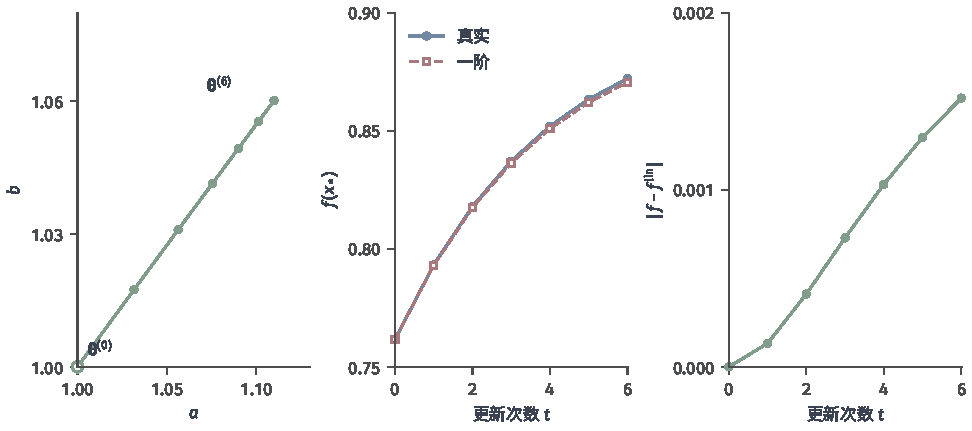
\includegraphics[width=164.600mm]{figures/03-foundations/02-learning-theory/matplotlib/learning-theory-ntk-linearization/figure.pdf}
  \caption{初始化附近的参数轨迹与输出线性化。教学神经网络为$f_{(a,b)}(x)=a\tanh(bx)$，
 初值为$(1,1)^\top$；用单个样本$(x,y)=(1,0.9)$的半平方损失、步长0.3执行六次
 梯度下降，连同初值共七个检查点。中间的真实输出和一阶输出均在左侧同一参数轨迹
 上计算；三面板绘图区大小相同，参数、输出和绝对余项各用所标坐标范围，不能按纸面高度直接比较数值。右侧余项末次约为0.00152。近初始化时二者接近，
 但余项并非零。参数增量经初始雅可比映射到输出／函数空间的切空间；NTK是初始梯度在不同输入上的内积。
 此有限神经网络示例展示近似对象，不证明训练中核恒定或新的预测输入上的误差受控。}
 \label{fig:learning-ntk-linearization}
\end{figure*}

在线性化模型中，训练只改变系数$\bm v$，神经网络的初始梯度特征保持为$\bm\varphi_0(\bm x)$。这个特征由神经网络和初始化决定，通常不是末层激活，也不是经验风险梯度。输出梯度只依赖输入，经验风险梯度还包含标签与当前预测误差。

从$\bm v=0$开始，每次经验风险梯度都是训练记录处初始梯度特征的线性组合，因此参数更新始终落在$\operatorname{span}\{\bm\varphi_0(\bm x_1),\ldots,\bm\varphi_0(\bm x_n)\}$这个子空间内。新的预测输入的初始梯度特征可以不在这个子空间，但它与训练记录处初始梯度特征的内积决定所学更新怎样影响预测。为表达这一传递关系，我们定义梯度内积对应的核。

\begin{definition}[神经切线核]
\label{def:neural-tangent-kernel}
设神经网络输出对参数可微。参数为$\bm\theta$时的神经切线核（neural tangent kernel, NTK）为
\[
 K_{\bm\theta}(\bm x,\bm x')=
 \left\langle\nabla_{\bm\theta}f_{\bm\theta}(\bm x),
               \nabla_{\bm\theta}f_{\bm\theta}(\bm x')\right\rangle.
\]
记$K_0=K_{\bm\theta^{(0)}}$，其在训练样本中的$n$个预测输入$\bm x_i$上的核矩阵为$\bm K_0$，其中
$(\bm K_0)_{i,j}=K_0(\bm x_i,\bm x_j)$。
\end{definition}

核值可以直接计算一次训练更新怎样传播到别的输入。若用第$i$条训练记录更新，损失对当前分数的导数为$a_i$，在线性化模型中
\[
 \Delta\bm v=-\eta a_i\bm\varphi_0(\bm x_i),\qquad
 \Delta f(\bm x_j)=-\eta a_i K_0(\bm x_j,\bm x_i).
\]
初始梯度方向相似时，在一条训练记录处更新参数，会同向地改变另一输入处的预测；两者正交时，这次更新对另一输入的预测没有影响。

沿用上面的教学例子，$K_0(1,1)\approx0.76^2+0.42^2\approx0.76$，$K_0(1,2)\approx0.76\times0.96+0.42\times0.14\approx0.79$。在$x=1$处做一次使输出升高0.1的更新，$x=2$处的输出也会升高约$0.1\times0.79/0.76\approx0.10$。也就是说，在这个神经网络看来，$x=1$和$x=2$非常相似，训练一个就几乎同等程度地改变另一个。这个结论只描述当前固定特征下的信息传递；特征一旦随训练改变，核值也随之改变。

图~\ref{fig:learning-ntk-features}将同一次更新分成两步：在训练记录$(\bm x_i,y_i)$处计算损失对参数的梯度，产生参数增量；再在另一预测输入$\bm x_j$处计算神经网络输出对参数的梯度，将增量转换为预测变化。图中的两份初始梯度特征均是神经网络输出对参数的梯度；训练记录处的损失梯度还要乘以损失对预测的导数，整份经验风险梯度还对训练记录求平均。

Jacot等在特定参数化、初始化和无限宽极限下得到确定核，并在相应训练条件下证明它保持不变\scite{jacot2018ntk}。神经网络由固定梯度特征描述时，常称为\term{惰性训练}（lazy training）。取宽度趋于无穷时，还需规定参数初始化的方差随宽度如何缩放：在一种缩放下核保持不变，换一种缩放则特征会在训练中持续变化。有限宽应用必须检查核变化与线性化余项；ReLU导数只在可微点直接使用，不可微点还需约定。

% 文献边注先随说明段排入侧栏，避免页底回移侵入跨栏图注。
\begin{figure*}[!htb]
  \centering
  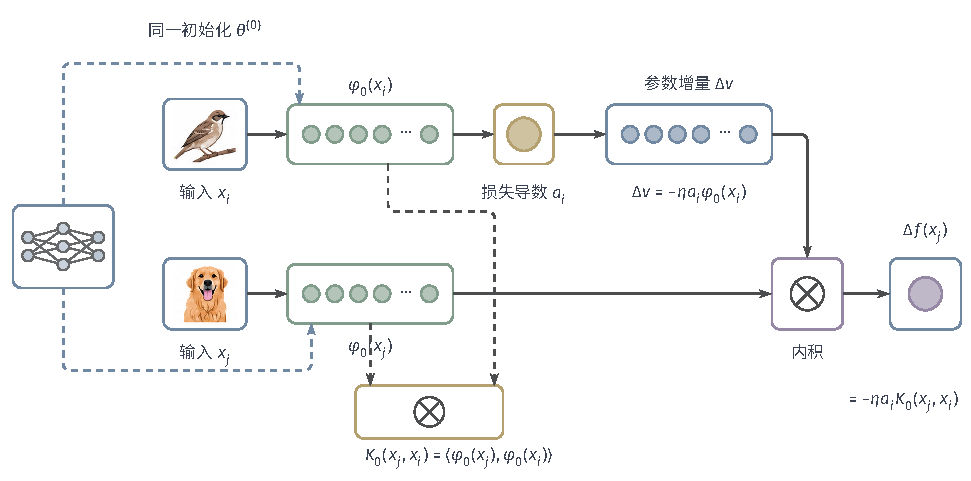
\includegraphics[width=164.600mm]{figures/03-foundations/02-learning-theory/tikz/learning-theory-ntk-features/figure.pdf}
  \caption{初始梯度特征如何传递一次训练更新。在线性化模型中，第$i$条训练记录的初始梯度特征与损失对预测的导数$a_i$共同确定参数增量$\Delta\bm v$；将同一增量与预测输入$\bm x_j$处的初始梯度特征作内积，得到$\Delta f(\bm x_j)$。核值$K_0$正是两个初始梯度特征的内积。蓝色虚线把两份梯度关联到同一初始化，深色虚线展示核内积所用的两份梯度。特征条仅示意梯度坐标，不限定参数维数。对真实有限宽神经网络使用固定特征，还需控制核变化与线性化误差。}
  \label{fig:learning-ntk-features}
\end{figure*}

\subsection{核矩阵与训练结果}

我们先用半平方损失计算训练样本上预测值的变化。令$\bm f(t)$和$\bm y$分别为训练样本上的预测与标签向量。梯度流下参数按$\dot{\bm\theta}=-\frac1n\sum_i(f_i-y_i)\nabla_{\bm\theta}f_i$变化，第$j$个预测的变化率为$\dot f_j=\langle\nabla_{\bm\theta}f_j,\dot{\bm\theta}\rangle=-\frac1n\sum_iK_{\bm\theta(t)}(\bm x_j,\bm x_i)(f_i-y_i)$。写成向量形式，就是真实神经网络的梯度流
\[
 \dot{\bm f}(t)=-\frac1n\bm K_{\bm\theta(t)}(\bm f(t)-\bm y).
\]
固定核模型将时间变化的矩阵换为$\bm K_0$，于是可以在各特征方向上求解。下面的定理要求$\bm K_0$正定。由于$\bm K_0$是$n$个初始梯度特征的Gram矩阵，正定等价于这些特征线性无关，必要条件是参数数$p\geq n$。过参数化在这里第一次起到正面作用：它使线性化模型有可能插值全部训练样本，这正是非凸训练仍能把损失降到零的一种解释。连续时间在此简化机制说明，离散更新还须检查步长。

\begin{theorem}[固定NTK下的训练收敛]
\label{thm:ntk-training-convergence}
设$n\geq1$，$\bm K_0\in\mathbb R^{n\times n}$为正定矩阵，
最小特征值为$\lambda_{\min}>0$，并给定
$\bm y,\bm f(0)\in\mathbb R^n$。若
$\dot{\bm f}(t)=-\bm K_0(\bm f(t)-\bm y)/n$，则
\[
 \bm f(t)-\bm y=e^{-\bm K_0t/n}(\bm f(0)-\bm y),
\]
并有
$\|\bm f(t)-\bm y\|_2\leq e^{-\lambda_{\min}t/n}\|\bm f(0)-\bm y\|_2$。
\end{theorem}
\begin{proof}
将$\bm K_0$正交对角化。特征值$\lambda_j$对应的残差分量满足
\[
 \dot e_j(t)=-\lambda_j e_j(t)/n,\qquad
 e_j(t)=e^{-\lambda_jt/n}e_j(0).
\]
合并各方向即得矩阵指数表达式，再用$\lambda_j\geq\lambda_{\min}$控制欧氏范数。
\end{proof}

预测残差在核矩阵各特征向量方向上的分量，按相应特征值决定的速率衰减：大特征值方向学得快，小特征值方向学得慢。例如取$n=2$，两个特征值分别为2和0.02。训练到$t=2$时，第一个方向的残差已乘上$e^{-2}\approx0.14$，第二个方向只乘上$e^{-0.02}\approx0.98$，几乎没动；要让第二个方向也缩到同样比例，训练时间须延长一百倍。相同训练时长下，标签在小特征值方向上的分量衰减最慢，因而主导剩余的训练误差。这个结论只约束训练样本上的预测误差；要分析新输入，还需确定训练最终得到哪个函数，以及它的复杂度有多大。

\subsection{再生核空间与期望风险}
\label{sec:ntk-rkhs-generalization}

训练收敛只回答了训练样本上的预测；要估计新输入上的风险，还要像上一节那样，用某种“大小”来衡量训练得到的函数，再由这个大小控制复杂度。线性化模型中最自然的候选是参数位移的欧氏范数$\|\bm v\|_2$，但它衡量的是参数，而风险只取决于函数。所以先要检查同一个线性化函数是否有不同参数表示。记所有允许输入的梯度特征张成的空间为$V_{\mathrm{all}}=\operatorname{span}\{\bm\varphi_0(\bm x):\bm x\in\mathcal X\}$。若$\bm u\in V_{\mathrm{all}}^\perp$，则$\langle\bm u,\bm\varphi_0(\bm x)\rangle=0$对每个输入成立，因而$\bm v$与$\bm v+\bm u$表示同一个线性化函数；参数范数却可能计入这个不改变函数的分量。全域特征空间是否为真子空间取决于架构和输入范围，不能只由参数多于训练样本推出：训练特征张成的$V_S$只满足$V_S\subseteq V_{\mathrm{all}}$，与$V_S$正交的位移仍可能改变新输入处的预测。固定核方法对同一函数的所有参数表示取最小范数，排除真正不影响函数的方向。即使$V_{\mathrm{all}}=\mathbb R^p$、没有这种冗余，下面的定义仍然成立，并等于唯一表示的欧氏范数。

由$K_0$生成的\term{再生核希尔伯特空间}（reproducing kernel Hilbert space, RKHS）记为$\mathcal H_{K_0}$。在当前问题中，可以把它理解为线性化模型能表示的全部函数增量，并配上一种“大小”：一个函数的大小，等于写出它所需的最短参数位移。在$\mathcal H_{K_0}$中，固定位置$\bm x$的核截面$K_0(\bm x,\cdot)$与函数的内积给出该函数在$\bm x$处的值；函数差的空间范数因而能够控制该位置的预测差异（可参考\BookVolumeRef{vol:mathematical-preliminaries-upper}{卷1《数学准备：计算、分析与几何》}）。在有限维梯度特征下，它包含$g(\bm x)=\langle\bm v,\bm\varphi_0(\bm x)\rangle$，并以
\[
 \|g\|_{\mathcal H_{K_0}}
 =\inf\{\|\bm v\|_2:g(\bm x)=\langle\bm v,\bm\varphi_0(\bm x)\rangle
                         \text{ 对所有 }\bm x\text{ 成立}\}
\]
计算函数复杂度。下确界排除了不影响函数的系数方向。我们控制的是相对于初始化的变化$g=f-f_0$，而非默认$f_0=0$后的整个输出。

由于控制对象是变化量$g$，若神经网络在初始化处的输出$f_0(\bm x)$并不为零，应先把初始预测从标签中减去，得到目标残差$r_i=y_i-f_0(\bm x_i)$和残差向量$\bm r=(r_1,\ldots,r_n)^\top$：若初始模型已经部分正确，训练只需补上剩余部分。从零参数位移出发，固定特征平方损失的梯度流在所有插值函数中选择最小RKHS范数者。下面将这个选解及其范数一起求出。

\begin{theorem}[初始梯度特征的最小范数插值]
\label{thm:ntk-minimum-rkhs-norm}
设$X$为非空集合，$K_0:X\times X\to\mathbb R$为正定核，
$\mathcal H_{K_0}$为其RKHS。给定$n\geq1$个输入$\bm x_1,\ldots,\bm x_n\in X$、
实数标签$y_1,\ldots,y_n$和函数$f_0:X\to\mathbb R$，定义
\[
 (\bm K_0)_{i,j}=K_0(\bm x_i,\bm x_j),\qquad
 r_i=y_i-f_0(\bm x_i),\qquad
 \bm r=(r_1,\ldots,r_n)^\top.
\]
假设核矩阵$\bm K_0$正定，并令
$\bm k_0(\bm x)=(K_0(\bm x_i,\bm x))_{i=1}^{n}$。
满足$g(\bm x_i)=r_i$的最小RKHS范数函数为
\[
 \widehat g(\bm x)=\bm k_0(\bm x)^\top\bm K_0^{-1}\bm r,
\]
其范数满足
\begin{equation}
 \|\widehat g\|_{\mathcal H_{K_0}}^2
 =\bm r^\top\bm K_0^{-1}\bm r
 =\sum_{j=1}^n\frac{(\bm u_j^\top\bm r)^2}{\lambda_j},
 \label{eq:ntk-label-spectral-complexity}
\end{equation}
其中$(\lambda_j,\bm u_j)$为$\bm K_0$的正交特征对。定义半平方经验损失
\[
 \mathcal E(g)=\frac1{2n}\sum_{i=1}^n
 \bigl(f_0(\bm x_i)+g(\bm x_i)-y_i\bigr)^2.
\]
对$\mathcal E$从$g_0=0$出发的RKHS梯度流
\[
 \dot g_t=-\frac1n\sum_{i=1}^n
 (f_0(\bm x_i)+g_t(\bm x_i)-y_i)K_0(\bm x_i,\cdot)
\]
收敛到$\widehat g$。
\end{theorem}
\begin{proof}
将任意$g$分解为$\operatorname{span}\{K_0(\bm x_i,\cdot)\}_{i=1}^n$中的分量与正交分量。由再生性质，正交分量在训练样本的各预测输入$\bm x_i$处取值为零，去掉它不改变插值条件，却不会增大范数。最小范数函数因而形如
$g=\sum_i a_iK_0(\bm x_i,\cdot)$。
插值条件为$\bm K_0\bm a=\bm r$，故$\bm a=\bm K_0^{-1}\bm r$，且
$\|g\|^2=\bm a^\top\bm K_0\bm a=\bm r^\top\bm K_0^{-1}\bm r$。
对核矩阵作谱分解得到第二个等式。梯度流始终留在上述张成空间中，训练收敛定理又保证插值，因此只能收敛到这个唯一的插值函数。
\end{proof}

式~\eqref{eq:ntk-label-spectral-complexity}按核特征方向计算插值代价：标签在特征值$\lambda_j$方向上的分量越大、$\lambda_j$越小，插值所需的范数就越大。所以小特征值本身不增加复杂度，只有标签确实需要沿这个方向变化时才付出代价。取
\[
 \bm K_0=\begin{pmatrix}1&1-a\\1-a&1\end{pmatrix},\qquad 0<a\leq1,
\]
其特征值为$2-a$（对应方向$(1,1)$，两输入同升同降）和$a$（对应方向$(1,-1)$，两输入一升一降）。残余标签同为1时，标签全在第一个方向上，范数平方为$2/(2-a)$，不超过2；标签为1和$-1$时，标签全在第二个方向上，范数平方却为$2/a$。取$a=0.01$，后者为200，是前者的约200倍。$a$小时，初始梯度把两输入判为几乎相同，强制它们取相反输出便需要很大的范数。核不变而标签方向改变，就足以改变复杂度及其风险界。

要把这一范数接到总体风险，我们固定独立于样本的核，并要求$K_0(\bm x,\bm x)\leq\kappa^2$，即梯度特征范数至多$\kappa$。再事先指定$B$，分析$\mathcal G_B=\{g\in\mathcal H_{K_0}:\|g\|_{\mathcal H_{K_0}}\leq B\}$的Rademacher复杂度。

\begin{theorem}[初始梯度特征的期望风险界]
\label{thm:ntk-rkhs-risk}
设$(X,\mathcal X)$为可测输入空间，$Y\subseteq\mathbb R$为可测标签空间，
$\mathcal P$为$X\times Y$上的概率分布，且
$S=((\bm x_1,y_1),\ldots,(\bm x_n,y_n))\sim\mathcal P^n$。
函数$f_0:X\to\mathbb R$与可测正定核$K_0:X\times X\to\mathbb R$
在抽样前确定；它们也可随机选取，但须与$S$独立，并且以下条件几乎必然成立。
令$\mathcal H_{K_0}$为$K_0$的RKHS，假设
$K_0(\bm x,\bm x)\leq\kappa^2$对所有$\bm x\in X$成立，并定义
\[
 \mathcal G_B=\{g\in\mathcal H_{K_0}:
                   \|g\|_{\mathcal H_{K_0}}\leq B\}.
\]
损失$\ell:\mathbb R\times Y\to[0,1]$可测，且关于第一个变量为
$G$-Lipschitz。对任意可测$f:X\to\mathbb R$，定义
\[
 R(f)=\mathbb E_{(\bm x,y)\sim\mathcal P}\ell(f(\bm x),y),\qquad
 \hat R_S(f)=\frac1n\sum_{i=1}^n\ell(f(\bm x_i),y_i).
\]
假设随机变量
$\sup_{g\in\mathcal G_B}|R(f_0+g)-\hat R_S(f_0+g)|$可测。
对任意在抽样前固定的$B,\kappa,G>0$和$\delta\in(0,1)$，以概率至少
$1-\delta$，对所有$g\in\mathcal G_B$同时有
\begin{equation}
 R(f_0+g)\leq\hat R_S(f_0+g)
       +\frac{2G\kappa B}{\sqrt n}
       +3\sqrt{\frac{\log(2/\delta)}{2n}}.
 \label{eq:ntk-rkhs-risk}
\end{equation}
若存在$g_\star\in\mathcal G_B$使
$y=f_0(\bm x)+g_\star(\bm x)$在$\mathcal P$下几乎处处成立，且
$\ell(y,y)=0$，并且样本核矩阵
$\bm K_0=(K_0(\bm x_i,\bm x_j))_{i,j=1}^n$几乎必然正定，则定义
\[
 \widehat g\in\argmin_{g\in\mathcal H_{K_0}}
 \left\{\|g\|_{\mathcal H_{K_0}}:
 f_0(\bm x_i)+g(\bm x_i)=y_i,\ 1\leq i\leq n\right\}.
\]
最小范数插值函数$\widehat g$满足同一上界且经验风险项为零。对任意
$\varepsilon\in(0,1)$，一个充分样本量条件是
\[
 n\geq\max\left\{\frac{16G^2\kappa^2B^2}{\varepsilon^2},
                  \frac{18\log(2/\delta)}{\varepsilon^2}\right\},
\]
此时期望风险以概率至少$1-\delta$不超过$\varepsilon$。
\end{theorem}
\begin{proof}
利用再生性质、Cauchy--Schwarz不等式以及独立随机正负号的交叉项期望为零，得到
\begin{align*}
 \widehat{\mathfrak R}_S(\mathcal G_B)
 &=\frac Bn\mathbb E_{\bm\sigma}
       \left\|\sum_{i=1}^n\sigma_i K_0(\bm x_i,\cdot)\right\|_{\mathcal H_{K_0}}\\
 &\leq\frac Bn\sqrt{\sum_{i=1}^nK_0(\bm x_i,\bm x_i)}
 \leq\frac{\kappa B}{\sqrt n}.
\end{align*}
固定$f_0$产生的偏移与所选函数无关，故不改变上述复杂度。再由损失的Lipschitz收缩性质引入因子$G$，应用有界损失的期望风险界，即得式~\eqref{eq:ntk-rkhs-risk}。

可实现函数$g_\star$满足所有插值条件，所以最小范数解满足$\|\widehat g\|\leq\|g_\star\|\leq B$，且经验风险为零。分别使风险界两项至多$\varepsilon/2$，就得到所列充分样本量。
\end{proof}

这个复杂度项与第~\ref{sec:rademacher-complexity}节线性分类器的结果形式相同：线性化模型就是以$\bm\varphi_0(\bm x)$为输入、以$\bm v$为系数的线性模型，$\kappa$对应输入长度上限，$B$对应系数范数上限。这条保证依赖四个条件：目标函数相对于初始化的变化能用小范数表示，核的对角值有界，样本独立同分布，以及训练确实达到对应的插值解。只要这些条件成立，即使特征维数无限，复杂度也由$\kappa B$控制；参数或特征的坐标个数在这里不单独决定风险。

谱与标签也可共同检验范数条件。式~\eqref{eq:ntk-label-spectral-complexity}说明，只要算出$\sum_j(\bm u_j^\top\bm r)^2/\lambda_j\leq B^2$，就知道插值解落在所控的范数球里。若这项条件另以概率至少$1-\delta_0$成立，两个事件的联合失败概率至多$\delta+\delta_0$。与上一节一样，$B$必须事先固定；若观察后才令$B=\|\widehat g\|$，需要对一列预定范数球同时控制，不能直接沿用原置信度。

核正定、即$\lambda_{\min}(\bm K_0)>0$，只保证能够插值，不能替代小范数条件。粗略界$\bm r^\top\bm K_0^{-1}\bm r\leq\|\bm r\|_2^2/\lambda_{\min}$中，标签平方和$\|\bm r\|_2^2$通常随样本数$n$线性增长；若最小特征值只保持常数，复杂度$B^2$也随$n$线性增长，代入风险界的$\kappa B/\sqrt n$后并不下降。要得到有意义的保证，必须像前面的二维例子那样，利用标签主要落在大特征值方向这一结构。Arora等对特定两层过参数化神经网络的分析同时使用标签与核谱，并在明确初始化、宽度和数据条件下得到训练及不显含宽度的样本复杂度保证\scite{arora2019finegrained}。

同一范数也可以经PAC--Bayes进入风险。这种方法不评价单个参数，而评价按某个分布随机抽取参数的预测器：训练前选定一个与样本无关的参数分布，称为先验；训练后选一个依赖样本的参数分布，称为后验。对有界损失，将后验与先验比较，相对熵记录后验偏离先验的代价，并与经验风险一起控制随机预测的总体风险（可参考\BookVolumeRef{vol:mathematical-preliminaries-lower}{卷2《数学准备：概率、因果与决策》}）。神经网络随机预测器版本见第~\ref{sec:pac-bayes}节。对有限维位移，事先取$P_0=\mathcal N(0,s^2\bm I_p)$、$s>0$，再以$Q=\mathcal N(\widehat{\bm v},s^2\bm I_p)$描述训练中心附近参数。相对熵为$\|\widehat{\bm v}\|_2^2/(2s^2)$。将定理~\ref{thm:pac-bayes-bound}与Lipschitz性合并，以概率至少$1-\delta$，所有中心同时有
\begin{equation}
 \begin{aligned}
 R(g_{\widehat{\bm v}})\leq{}&\hat R_S(g_{\widehat{\bm v}})+2Gs\kappa\\
 &+\sqrt{\frac{\|\widehat{\bm v}\|_2^2/(2s^2)+\log((n+1)/\delta)}{2n}},
 \end{aligned}
 \label{eq:ntk-pac-bayes-risk}
\end{equation}
其中$g_{\bm v}=f_0+\langle\bm v,\bm\varphi_0\rangle$。投影扰动$\langle\bm v-\widehat{\bm v},\bm\varphi_0(\bm x)\rangle$的绝对值期望至多$s\kappa$，把随机预测的经验与总体风险分别转回中心各付出$Gs\kappa$。最小范数表示满足$\|\widehat{\bm v}\|_2^2=\|\widehat g\|_{\mathcal H_{K_0}}^2$，因此同一核谱量出现在信息代价中。

PAC--Bayes在这里引入一个新的取舍。$s$表示训练中心周围随机扰动的幅度：增大$s$，后验与先验更接近，信息代价$\|\widehat{\bm v}\|_2^2/(2s^2)$减小；但扰动越大，随机预测器偏离中心越远，扰动损失$2Gs\kappa$增大。若插值范数统一有界，预先取$s_n=n^{-1/4}$可使两项都随$n$下降，但这个简单构造的速率可能比Rademacher界慢。各向同性高斯只在有限维参数空间中直接可用；无限维RKHS中不存在协方差为$s^2I$的同类概率分布，此时仍可采用前面的复杂度证明。

\subsection{正则化、稳定性与有限宽度}

固定梯度特征之后，模型对参数$\bm v$是线性的，训练目标对凸损失便是凸函数，可以直接使用凸学习的稳定性分析。前面的范数路线控制整个函数空间；稳定性路线则比较两份相邻样本训练出的输出。需要注意，“一次训练中核变化很小”说的是同一次训练随时间的变化，并没有说明两份只差一个样本的训练集会得到相近的函数，二者不能互相替代。

对$g_{\bm v}(\bm x)=f_0(\bm x)+\langle\bm v,\bm\varphi_0(\bm x)\rangle$加入二次惩罚，就可沿第~\ref{sec:regularized-learning}节比较相邻样本的最优解。这里固定与样本独立的初始化，并要求$\|\bm\varphi_0(\bm x)\|_2\leq\kappa$。

\begin{theorem}[正则化固定特征模型的稳定性]
\label{thm:ntk-stability-risk}
设$(X,\mathcal X)$为可测输入空间，$(Y,\mathcal Y)$为可测标签空间，
$\mathcal P$为$X\times Y$上的概率分布，且
$S=((\bm x_1,y_1),\ldots,(\bm x_n,y_n))\sim\mathcal P^n$。
在抽样前固定可测函数$f_0:X\to\mathbb R$和
$\bm\varphi_0:X\to\mathbb R^p$，其中
$\|\bm\varphi_0(\bm x)\|_2\leq\kappa$对所有$\bm x\in X$成立，并令
$g_{\bm v}(\bm x)=f_0(\bm x)+\langle\bm v,\bm\varphi_0(\bm x)\rangle$。
设损失$\ell:\mathbb R\times Y\to\mathbb R$可测，关于第一个变量凸且为
$G$-Lipschitz，并满足
$\mathbb E_{(\bm x,y)\sim\mathcal P}|\ell(f_0(\bm x),y)|<\infty$。
定义
\[
 R(g_{\bm v})=\mathbb E_{(\bm x,y)\sim\mathcal P}
                    \ell(g_{\bm v}(\bm x),y),\qquad
 \hat R_S(g_{\bm v})=\frac1n\sum_{i=1}^n
                    \ell(g_{\bm v}(\bm x_i),y_i).
\]
对$G,\kappa,\lambda>0$，令
\[
 \widehat{\bm v}_S=\argmin_{\bm v}
 \left\{\frac1n\sum_{i=1}^n\ell(g_{\bm v}(\bm x_i),y_i)
       +\frac\lambda2\|\bm v\|_2^2\right\},\qquad\lambda>0.
\]
则算法的均匀稳定性至多为$2G^2\kappa^2/(\lambda n)$，且对任意固定
$\bm v\in\mathbb R^p$，
\[
 \mathbb E_S R(g_{\widehat{\bm v}_S})-R(g_{\bm v})
 \leq\frac{2G^2\kappa^2}{\lambda n}+\frac\lambda2\|\bm v\|_2^2.
\]
\end{theorem}
\begin{proof}
单个样本损失关于$\bm v$为$G\kappa$-Lipschitz，经验目标为$\lambda$-强凸。定理~\ref{thm:regularized-erm-stability}给出替换一个样本后的参数距离上界$2G\kappa/(\lambda n)$，再乘损失的Lipschitz常数即得均匀稳定性及期望泛化差上界。正则化最优性还保证
\[
 \hat R_S(g_{\widehat{\bm v}_S})
 \leq\hat R_S(g_{\bm v})+\frac\lambda2\|\bm v\|_2^2.
\]
对样本取期望，并使用固定$\bm v$的经验风险期望等于期望风险，得到结论。
\end{proof}

指定比较半径$B>0$，取$\lambda=2G\kappa/(B\sqrt n)$，得到
\begin{equation}
 \mathbb E_S R(g_{\widehat{\bm v}_S})
 -\inf_{\|\bm v\|_2\leq B}R(g_{\bm v})
 \leq\frac{2G\kappa B}{\sqrt n}.
 \label{eq:ntk-sample-risk}
\end{equation}
这个选择平衡两种代价：$\lambda$越大，替换一个样本时解的变化越小（稳定性代价$2G^2\kappa^2/(\lambda n)$下降），但正则化把解拉得离最优比较参数越远（比较代价$\lambda B^2/2$上升）。令两项相等即得上述$\lambda$。小特征值方向的变化还可以在平方损失的一个独立例子中看清。令$r_i=y_i-f_0(\bm x_i)$，单独考虑目标
\[
 \frac1{2n}\sum_{i=1}^n
 \bigl(\langle\bm v,\bm\varphi_0(\bm x_i)\rangle-r_i\bigr)^2
 +\frac\lambda2\|\bm v\|_2^2.
\]
用原始Gram矩阵$\bm K_0$、残差向量$\bm r$记系数，最优参数可写为$\bm v=\sum_i\alpha_i\bm\varphi_0(\bm x_i)$，其中$\bm\alpha=(\bm K_0+n\lambda\bm I)^{-1}\bm r$。若$\bm K_0\bm u_j=\lambda_j\bm u_j$，残差的第$j$个特征分量在该系数中乘以$1/(\lambda_j+n\lambda)$，训练预测分量则乘以$\lambda_j/(\lambda_j+n\lambda)$。因此正则化限制了小特征值带来的系数放大；只有改用$\bm K_0/n$的特征值时，分母才相应写成归一化特征值加$\lambda$。这里的$n$来自经验目标取样本平均，不能省略。

平方损失并非全局Lipschitz，上述谱计算只是解释正则化作用的代数例子，不能直接套入刚才的凸Lipschitz稳定性定理。该定理给出平均意义的保证，前面的Rademacher结论要求有界Lipschitz损失并给出高概率保证，二者仍须按各自条件使用。

以上结论都针对固定特征的线性化模型，真实有限宽神经网络还需从线性化模型转回实际输出。记二者训练后得到的函数分别为$f_S$和$g_S$。若以概率至少$1-\delta_{\mathrm{app}}$（对样本、初始化及算法随机性）满足
\[
 \mathbb E_{\bm x\sim\mathcal P_X}|f_S(\bm x)-g_S(\bm x)|\leq\tau_n,
\]
则$G$-Lipschitz损失把两者期望风险之差控制在$G\tau_n$以内。对$\mathcal P_X$几乎处处一致的$\tau_n$界同样足够；近似成功的事件需与复杂度事件一起计入失败概率。只知道训练样本处的核矩阵变化很小，还没有证明新输入上的这个误差也小。因此完整的风险保证同时依赖复杂度、训练拟合与近似误差三部分。若训练中特征明显改变，线性化就不再适用，需要转向分析整个更新过程。

\section{基于参数梯度更新的可学习性}
\label{sec:implicit-bias}

固定初始梯度路线只适用于特征在训练中几乎不变的情形。然而，神经网络相对于固定核方法的主要优势，恰恰被认为来自训练中学到的特征；把特征冻结在初始化处，就把这部分机制排除在分析之外。一般的训练会改变这些特征，参数化方式和优化器也会影响最终选出哪个解。我们于是把分析对象从“初始化处的局部响应”改为“从初始化到训练结束的整条参数轨迹”，研究这条轨迹如何决定最终函数。非线性神经网络的完整轨迹难以求解，所以本节在线性回归、线性分类和深层线性神经网络这几类能够算清的模型中证明选解机制，再说明结论能推广到哪里。

从离散的梯度下降写法看，固定步长时参数的全部更新累加为
\[
 \bm\theta^{(t)}=\bm\theta^{(0)}
 -\eta\sum_{s=0}^{t-1}\nabla_{\bm\theta}\hat R_S(\bm\theta^{(s)}).
\]
每一步的梯度都在此前更新到达的位置上计算，因此各步互相依赖：最终停在哪里，取决于从哪里出发、走过怎样的路径。同一个函数用不同方式参数化，梯度路径也会不同。一个最简单的例子是标量模型$wx$。直接训练$w$时，若损失对$w$的梯度为$g$，每步更新量都是$-\eta g$，与$w$当前的大小无关；改写成$w=uv$后，$u$的更新量是$-\eta gv$，$v$的更新量是$-\eta gu$，于是$w$本身的变化约为$-\eta g(u^2+v^2)$。系数已经较大时变化更快，接近零时几乎不动。两种写法表示同一族函数，训练却会走出不同的路线。\term{梯度动力学}（gradient dynamics）研究这些连续更新怎样决定最终函数。

这种由初始化、损失、参数化和更新规则共同产生、但没有显式写进目标函数的选解倾向，称为\term{隐式偏差}（implicit bias）。这里的“偏差”指算法偏好某一类解，不是风险分解中的近似误差，也不是某一次更新本身；“隐式”则强调这种偏好没有通过正则化项等方式显式声明。上面的$w=uv$例子已经显示了它的来源：同一族函数换一种参数化，更新的快慢分配就不同，最终停下的位置也随之不同。

知道算法偏好什么解，还不等于有风险保证。我们可以先证明所选解具有受控的范数、间隔或谱结构，再套用复杂度界或直接计算风险；也可以比较两份相邻样本训练出的最终输出，直接用稳定性控制泛化差。

\subsection{参数更新、隐式偏差与泛化路径}

下面用三个可以算清楚的场景观察更新怎样选解：平方损失线性回归中，梯度下降收敛到一个有限的最小范数解；线性可分的逻辑分类中，参数范数无限增长，方向却趋于最大间隔方向；矩阵分解的梯度流则改变端到端矩阵奇异值的增长方式。三个场景是并列的机制，不是连续步骤，也不会统一导向同一种范数。每个场景都需要自己的数据与泛化条件。

这些分析都回到式~\eqref{eq:deep-risk-decomposition}。若更新选出了受控的几何结构，就用相应风险界控制泛化差；若映射$S\mapsto A(S)$本身稳定，就直接用稳定性界。算法带有随机性时，平均还要包括算法内部的随机数。接下来的三个场景走前一条路线，最后一个小节讨论后一条路线。

\subsection{最小范数与线性回归泛化}

本节开头已用一个训练样本$\bm x=(1,1)^\top$、$y=1$的例子说明：插值要求$w_1+w_2=1$，直线上的$(1,0)^\top$、$(0,1)^\top$和$(1/2,1/2)^\top$都能拟合，却在新输入$(1,0)^\top$上分别预测1、0与$1/2$。零初始化时，梯度$(w_1+w_2-1)(1,1)^\top$的两个分量始终相同，轨迹保持$w_1=w_2$，只能趋于中点。直线上其他点可写成$(1/2+a,1/2-a)^\top$，范数平方为$1/2+2a^2$，所以中点正是范数最小者。

图~\ref{fig:learning-minimum-norm}在参数平面画出这条插值直线。零初始化轨迹沿$w_1=w_2$抵达离原点最近的点；直线其余点也满足训练约束，却对同一个新预测输入给出不同预测。图只固定了选解，还没有给出该预测输入对应的真实标签。

\begin{figure}[htbp]
  \centering
  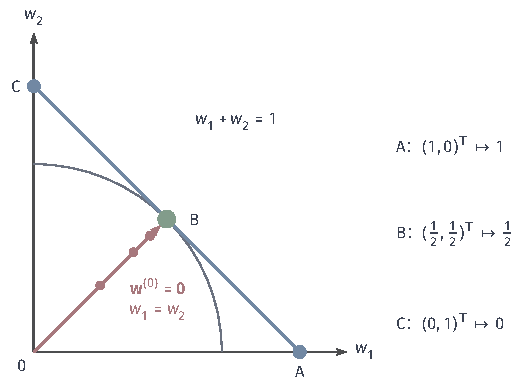
\includegraphics[width=88.805mm]{figures/03-foundations/02-learning-theory/tikz/learning-theory-minimum-norm/figure.pdf}
  \caption{一个训练观测对应多个插值参数。直线上的A、B、C都使输入$(1,1)^\top$的预测为1，
 右侧列出它们对同一个新预测输入$\bm x_{\mathrm{new}}=(1,0)^\top$的预测。对半平方损失从零初始化，图中以步长$1/4$
 画出前三次更新，轨迹趋向B；细弧表示经过B的欧氏范数等值线，说明B是插值直线上
 距离原点最近的点。这个教学例子解释选解规则，不给出新的预测输入的真实标签或泛化保证。}
 \label{fig:learning-minimum-norm}
\end{figure}
\FloatBarrier

\begin{theorem}[梯度下降的最小范数选择]
\label{thm:learning-gradient-descent-minimum-norm}
设$n,d\geq1$且$d>n$，$\bm X\in\mathbb R^{n\times d}$满行秩，
$\bm y\in\mathbb R^n$。对
$\hat R_S(\bm w)=\|\bm X\bm w-\bm y\|_2^2/(2n)$，令
\[
 \bm w^{(t+1)}=\bm w^{(t)}-\eta\nabla\hat R_S(\bm w^{(t)}),
 \qquad \bm w^{(0)}=0.
\]
若步长$0<\eta<2n/\|\bm X\|_2^2$，则
\begin{equation}
 \bm w^{(t)}\longrightarrow\hat{\bm w}
 =\bm X^\top(\bm X\bm X^\top)^{-1}\bm y
 =\argmin_{\bm X\bm w=\bm y}\|\bm w\|_2.
 \label{eq:learning-minimum-norm-interpolator}
\end{equation}
\end{theorem}
\begin{proof}
证明分两步。第一步说明迭代始终在训练输入张成的行空间$\operatorname{range}(\bm X^\top)$内：每次更新的增量都是$-\eta\bm X^\top(\bm X\bm w^{(t)}-\bm y)/n$，即$\bm X$各行的线性组合，而初值为零，所以以后每一步都不会产生与训练输入正交的分量。第二步证明残差趋于零。令$\bm e^{(t)}=\bm X\bm w^{(t)}-\bm y$，则
\[
 \bm e^{(t+1)}=
 \left(\bm I-\frac\eta n\bm X\bm X^\top\right)\bm e^{(t)}.
\]
满行秩使$\bm X\bm X^\top$正定；步长条件使括号内全部特征值的绝对值小于1，所以$\bm e^{(t)}\to0$，即迭代收敛到一个插值解。行空间中的插值解唯一，正是式~\eqref{eq:learning-minimum-norm-interpolator}中的$\hat{\bm w}$。任意其他插值解均可写成
\begin{equation}
 \bm w=\hat{\bm w}+\bm v,\qquad\bm v\in\operatorname{null}(\bm X).
 \label{eq:learning-interpolator-decomposition}
\end{equation}
行空间与零空间正交，故$\|\bm w\|_2^2=\|\hat{\bm w}\|_2^2+\|\bm v\|_2^2$，当且仅当$\bm v=0$时范数最小。这证明了最小范数性质。
\end{proof}

证明的核心是一个几何事实：梯度$\bm X^\top(\cdot)$总落在训练输入张成的行空间里，所以从零出发的迭代永远不会获得零空间方向上的分量。零初始化正是排除了这种分量；若初值已经带有零空间分量，梯度不会消除它，极限也就未必是最小范数解——在上面的二维例子中，从$(1,0)^\top$出发时迭代一步不动，因为它本身已经插值。这一结论只针对线性模型的欧氏范数，深层参数化会改变同一函数的参数表示和范数定义，因而不能把结论直接推广到全部神经网络。

确定最小范数解后，还要回答它在新输入上的误差有多大。定理~\ref{thm:learning-gradient-descent-minimum-norm}解决了“训练选哪个解”，但同一个最小范数解在不同数据分布下的表现可以很不相同：若真实关系恰好落在训练样本张成的方向上，误差就小；若真实关系主要在训练样本看不到的方向上，误差就大。因此这里不能再沿用只看假设空间复杂度的思路，而要在一个明确的数据生成模型下，把误差的来源一项项算清。

先固定数据模型。假设存在真实参数$\bm w_\star$，标签由$y=\bm x^\top\bm w_\star+\xi$生成，其中噪声$\xi$与输入独立、均值为零、方差为$\sigma^2$；再记输入的未中心化二阶矩矩阵$\bm\Sigma=\mathbb E[\bm x\bm x^\top]$，它记录输入在各个方向上的平方规模。若$\mathbb E\bm x=0$，它也等于协方差矩阵；这里的风险恒等式只需二阶矩有限，并不额外要求输入均值为零。风险采用完整平方损失$(\bm x^\top\bm w-y)^2$；前面优化用的半平方损失只差常数因子，不改变最小范数极限。对任意固定的$\bm w$，新观测误差可写为$\bm x^\top\bm w-y=\bm x^\top(\bm w-\bm w_\star)-\xi$。平方后取期望，交叉项$\mathbb E[\xi\,\bm x^\top(\bm w-\bm w_\star)]$因噪声在给定输入时均值为零而消失，于是$R(\bm w)=(\bm w-\bm w_\star)^\top\bm\Sigma(\bm w-\bm w_\star)+\mathbb E\xi^2$；取$\bm w=\bm w_\star$得$R(\bm w_\star)=\mathbb E\xi^2$。两式相减得到一个关键事实：
\[
 R(\bm w)-R(\bm w_\star)
 =\|\bm w-\bm w_\star\|_{\bm\Sigma}^2,
 \qquad\|\bm v\|_{\bm\Sigma}^2=\bm v^\top\bm\Sigma\bm v.
\]
也就是说，回归超额风险恰好等于参数误差在输入二阶矩矩阵下的加权长度，而不是参数的欧氏长度。这个加权距离按输入实际出现的方向评价参数误差：参数在输入很少出现的方向上偏差再大，对预测的影响也很小。因此仅看欧氏距离不能确定预测风险。

\begin{theorem}[基于最小范数的回归期望风险]
\label{thm:minimum-norm-risk-decomposition}
设$\bm x\in\mathbb R^d$为满足
$\mathbb E\|\bm x\|_2^2<\infty$的测试样本中的预测输入，
$\bm\Sigma=\mathbb E[\bm x\bm x^\top]$。给定
$\bm w_\star\in\mathbb R^d$，令测试标签
$y=\bm x^\top\bm w_\star+\xi$，其中
$\mathbb E[\xi\mid\bm x]=0$且$\mathbb E[\xi^2]<\infty$，并用完整平方损失定义
\[
 R(\bm w)=\mathbb E[(\bm x^\top\bm w-y)^2].
\]
固定满行秩设计矩阵$\bm X\in\mathbb R^{n\times d}$，其中$n<d$，
训练标签为$\bm y=\bm X\bm w_\star+\bm\xi$，
其中$\mathbb E[\bm\xi\mid\bm X]=0$、
$\mathbb E[\bm\xi\bm\xi^\top\mid\bm X]=\sigma^2\bm I_n$且$\sigma^2\geq0$。
令$\hat{\bm w}=\bm X^\top(\bm X\bm X^\top)^{-1}\bm y$，
$\bm P_X=\bm X^\top(\bm X\bm X^\top)^{-1}\bm X$。则
\begin{equation}
 \begin{aligned}
 &\mathbb E_{\bm\xi\mid\bm X}
       [R(\hat{\bm w})-R(\bm w_\star)]\\
 &\quad=\|(\bm I-\bm P_X)\bm w_\star\|_{\bm\Sigma}^2
 +\sigma^2\operatorname{tr}\left[
 \bm\Sigma\bm X^\top(\bm X\bm X^\top)^{-2}\bm X\right].
 \end{aligned}
 \label{eq:minimum-norm-prediction-risk}
\end{equation}
\end{theorem}
\begin{proof}
证明的第一步先把最小范数解分解成两部分。把训练标签$\bm y=\bm X\bm w_\star+\bm\xi$代入
\[\hat{\bm w}=\bm X^\top(\bm X\bm X^\top)^{-1}\bm y=\bm P_X\bm w_\star+\bm X^\top(\bm X\bm X^\top)^{-1}\bm\xi,
\]
其中$\bm P_X=\bm X^\top(\bm X\bm X^\top)^{-1}\bm X$是向训练输入张成空间的正交投影矩阵。于是
\[\hat{\bm w}-\bm w_\star=-(\bm I-\bm P_X)\bm w_\star+\bm X^\top(\bm X\bm X^\top)^{-1}\bm\xi.
\]
第一项与噪声无关，只由真实参数和训练样本覆盖的方向决定；第二项含噪声，是训练标签中的随机波动被写进了参数。在$\bm\Sigma$半范数下展开平方，条件噪声均值为零使两项交叉项期望为零，噪声项记$\bm M=\bm X^\top(\bm X\bm X^\top)^{-1}$，则$\mathbb E\|\bm M\bm\xi\|_{\bm\Sigma}^2=\mathbb E\operatorname{tr}(\bm\Sigma\bm M\bm\xi\bm\xi^\top\bm M^\top)=\sigma^2\operatorname{tr}(\bm\Sigma\bm M\bm M^\top)$，其中用到$\mathbb E[\bm\xi\bm\xi^\top\mid\bm X]=\sigma^2\bm I$；而$\bm M\bm M^\top=\bm X^\top(\bm X\bm X^\top)^{-2}\bm X$，就得到迹表达式。
\end{proof}

若设计矩阵也随机且式~\eqref{eq:minimum-norm-prediction-risk}右侧可积，再对$\bm X$平均即可包括全部训练随机性。两项误差各有直观含义。第一项来自训练样本没有覆盖的方向：$\bm P_X$是向训练输入张成空间的投影，$(\bm I-\bm P_X)\bm w_\star$是真实参数在训练样本完全看不到的那部分，零初始化不会凭空补出它，最小范数解在这些方向上干脆取零。在二维例子中，若真实参数是$\bm w_\star=(1,0)^\top$，训练样本只看到它在$(1,1)$方向的投影，模型学到$(1/2,1/2)^\top$，在$(1,-1)$方向上丢失了$(1/2,-1/2)^\top$这一部分。第二项来自拟合训练噪声：矩阵$(\bm X\bm X^\top)^{-1}$在训练输入接近线性相关的方向上很大，会把这些方向上的噪声放大后写进参数。最小范数选择本身两项都排除不了。零一风险的范数界也不能替代这里平方损失下的分布计算。

输入二阶矩矩阵的特征值分布决定上面两类误差对预测风险的影响大小：若遗漏的方向和噪声被放大的方向恰好都是输入很少出现的方向，它们对风险的影响就很小。Bartlett等的良性过拟合分析说明，在特定的特征值条件下，最小范数插值可以一边拟合噪声、一边保持小超额风险\scite{bartlett2020benign}。因此样本量分析必须同时说明算法选解和数据分布，不能只另换一个参数计数公式。

一个精确例子取无噪声和各向同性输入：$\bm x_i\sim\mathcal N(0,\bm I_d)$，$\sigma=0$，故$\bm\Sigma=\bm I_d$。随机$n$维样本子空间具有旋转对称性，期望投影只能是单位矩阵的倍数；由$\operatorname{tr}(\bm P_X)=n$可知$\mathbb E\bm P_X=(n/d)\bm I_d$。于是
\begin{equation}
 \mathbb E_S[R(\hat{\bm w})-R(\bm w_\star)]
 =\left(1-\frac nd\right)\|\bm w_\star\|_2^2,
 \qquad n<d.
 \label{eq:isotropic-minimum-norm-risk}
\end{equation}
$\|\bm w_\star\|_2=1,d=100,n=10$时，经验风险为零而平均超额风险为0.9。由精确式，使风险至多$\varepsilon<1$需要$n\geq d(1-\varepsilon)$。这个例子保留了维度影响，显示最小范数不会自动消除未观察方向的误差。

\subsection{最大间隔与线性分类泛化}

逻辑分类与平方回归的参数极限不同。对线性可分数据，把参数沿正确分类的方向不断放大，每个样本的$y\bm w^\top\bm x$都会变大，$\log(1+e^{-y\bm w^\top\bm x})$便持续下降。经验风险的下确界为零，却没有哪个有限参数能达到它，所以梯度下降会让参数范数一直增长。参数向量本身不收敛，有意义的问题变成：归一化后的参数方向$\bm w/\|\bm w\|_2$会趋于哪里？由于分类结果只取决于方向，这个问题也正是“最终得到哪条分类边界”。

取$y_i\in\{-1,1\}$，可分要求存在$\bm w$使所有$y_i\bm w^\top\bm x_i>0$。单位方向$\bm u$满足$\|\bm u\|_2=1$，其最小经验间隔为$\min_i y_i\bm u^\top\bm x_i$，即离分类边界最近的训练样本到边界的距离。把未归一化间隔固定为至少1后最小化范数，等价于最大化单位方向的这个最小距离，得到硬间隔支持向量机的几何目标：在所有能分开训练样本的边界中，选离两类最近样本都最远的那一条。

\begin{theorem}[逻辑回归梯度下降的最大间隔方向]
\label{thm:logistic-max-margin-direction}
设$n,d\geq1$，$\bm x_i\in\mathbb R^d$、$y_i\in\{-1,+1\}$，
且存在$\bm w\in\mathbb R^d$使
$y_i\bm w^\top\bm x_i>0$对所有$1\leq i\leq n$成立。
令$\bm X\in\mathbb R^{n\times d}$以$\bm x_i^\top$为第$i$行，并定义
\[
 \hat R_S(\bm w)=\frac1n\sum_{i=1}^{n}
             \log(1+e^{-y_i\bm w^\top\bm x_i})
\]
以及迭代
\[
 \bm w^{(t+1)}=\bm w^{(t)}-\eta\nabla\hat R_S(\bm w^{(t)}).
\]
从任意$\bm w^{(0)}\in\mathbb R^d$出发，取
$0<\eta<n/\|\bm X\|_2^2$。则$\|\bm w^{(t)}\|_2\to\infty$，且
\[
 \frac{\bm w^{(t)}}{\|\bm w^{(t)}\|_2}
 \longrightarrow\frac{\widehat{\bm w}_{\mathrm{svm}}}
                         {\|\widehat{\bm w}_{\mathrm{svm}}\|_2},
\]
其中
\[
 \widehat{\bm w}_{\mathrm{svm}}
 =\argmin_{\bm w}\tfrac12\|\bm w\|_2^2
 \quad\text{满足}\quad y_i\bm w^\top\bm x_i\geq1\quad(1\leq i\leq n).
\]
\end{theorem}
以下证明采用Soudry等对可分逻辑回归证明的渐近展开\scite{soudry2018implicit}。
\begin{proof}[证明（使用外部渐近结果）]
在上述保守步长条件下，
$\bm w^{(t)}=\widehat{\bm w}_{\mathrm{svm}}\log t+\bm\rho^{(t)}$，其中
$\|\bm\rho^{(t)}\|_2=O(\log\log t)$。
由于$\log\log t/\log t\to0$，除以$\log t$后取极限得到$\widehat{\bm w}_{\mathrm{svm}}$。该向量非零，故参数范数发散，并且归一化方向收敛到所述方向。这里的渐近展开是所引用的外部结果，本段只证明由该展开到方向收敛的推论。
\end{proof}

我们可以从每个样本对梯度的贡献理解这一方向选择：
\[
 -\nabla\hat R_S(\bm w)
 =\frac1n\sum_{i=1}^{n}
       \frac{y_i\bm x_i}{1+e^{y_i\bm w^\top\bm x_i}}.
\]
样本$i$的贡献由系数$1/(1+e^{y_i\bm w^\top\bm x_i})$控制。这个系数随分类间隔快速衰减：间隔为0时系数为0.5，间隔为1时约为0.27，间隔为5时只剩约0.0067。随着参数范数增长，离边界远的样本间隔越来越大，对更新方向的影响迅速消失；离边界最近的几个样本衰减最慢，最终主导更新方向。梯度下降于是不断调整方向，使这些最近样本离边界更远，这正是最大间隔方向的含义，也与支持向量机只由支持向量决定的性质对应。这里的系数由当前预测计算得到，并不是额外需要训练的参数。即使所有训练样本都已分对，逻辑损失仍会推动参数方向变化。这个机制解释不能替代方向极限的渐近证明。

最大间隔方向可以通过前面的复杂度理论转为期望风险保证。
\begin{theorem}[基于最大间隔的分类期望风险]
\label{thm:max-margin-classification-risk}
设$X\subseteq\mathbb R^d$取Borel $\sigma$代数，$Y=\{-1,+1\}$，
$\mathcal P$为$X\times Y$上的概率分布。令
\[
 S=((\bm x_1,y_1),\ldots,(\bm x_n,y_n))\sim\mathcal P^n.
\]
假设$\|\bm x\|_2\leq r$在$\mathcal P$下几乎处处成立，其中$n\geq1$、$r>0$。
事先固定$\gamma>0$和$\delta\in(0,1)$。则以概率至少$1-\delta$，所有满足
$\|\bm u\|_2=1$的方向同时满足
\begin{equation}
 \begin{aligned}
 \mathbb P_{(\bm x,y)\sim\mathcal P}\{y\bm u^\top\bm x\leq0\}
 \leq{}&\frac1n\sum_{i=1}^n
       \mathbb I\{y_i\bm u^\top\bm x_i\leq\gamma\}\\
 &+\frac{2r}{\gamma\sqrt n}
       +3\sqrt{\frac{\log(2/\delta)}{2n}}.
 \end{aligned}
 \label{eq:gradient-direction-margin-risk}
\end{equation}
左侧把零分数也计为错误，因而上界任意固定平局规则下的零一损失期望风险。
\end{theorem}
\begin{proof}
单位范数线性函数类的经验Rademacher复杂度至多为$r/\sqrt n$。
取在负间隔处为1、从0到$\gamma$线性下降、在不小于$\gamma$处为0的间隔损失。
它以$1/\gamma$为Lipschitz常数，上界控制零一损失，而它在训练样本上的取值又不超过
$\mathbb I\{y_i\bm u^\top\bm x_i\leq\gamma\}$。
对该损失应用Rademacher复杂度的Lipschitz收缩和统一期望风险界，即得结论。
\end{proof}

若训练数据的最大归一化间隔大于预定的$\gamma$，定理~\ref{thm:logistic-max-margin-direction}保证充分训练后的方向也达到这一阈值，式~\eqref{eq:gradient-direction-margin-risk}的经验项便为零。余项不超过$\varepsilon$的充分样本量为$O((r^2/\gamma^2+\log(1/\delta))/\varepsilon^2)$量级。例如输入归一化为$r=1$、预定阈值$\gamma=0.1$，且训练样本最大归一化间隔严格大于0.1时，复杂度项为$2/(0.1\sqrt n)$，要降到0.05需要$n\geq1.6\times10^5$；与输入维数$d$无关。

真正进入风险的是归一化间隔。统一放大参数会同时放大原始间隔和范数，不改变两者之比；只有方向变化才可能改善它。样本可分也不保证随$n$增长仍有固定的正间隔：若数据带有标签噪声，靠记忆噪声样本得到的可分边界间隔可能很小，界也随之失效。标签噪声、优化器或深层参数化改变时，都要重新证明选解性质。

\subsection{谱偏好与矩阵预测的泛化}

深层线性神经网络没有激活函数，表示的仍是线性映射，却已经足以显示参数化怎样改变选解。$\bm W=\bm W_L\cdots\bm W_1$给出线性输出$\bm W\bm x$。不同的分解可以表示同一映射，但对每个因子求梯度时都会乘上其余因子，所以训练路径依赖于分解方式，可以偏向不同的端到端映射；参数目标也因此可能非凸。

这类问题的典型应用是矩阵补全。考虑一个$1000\times1000$的用户—电影评分矩阵，但只观测到约1\%的元素，任务是预测其余元素。满足所有观测值的矩阵有无穷多个，问题与欠定线性回归一样需要选解；若用户偏好主要由题材、年代等少数因素决定，真实评分矩阵近似低秩，偏好低秩解的算法就更可能猜对未观测元素。下面要说明，分解参数化会让梯度流偏好奇异值集中在少数方向的解。

先用二层分解$\bm W=\bm U\bm V^\top$计算这项区别。记经验目标$\mathcal L(\bm W)$及梯度$\bm G=\nabla_{\bm W}\mathcal L$，链式法则给出
\[
 \dot{\bm U}=-\bm G\bm V,\qquad
 \dot{\bm V}=-\bm G^\top\bm U.
\]
从而
\begin{equation}
 \dot{\bm W}=-\bm G\bm V\bm V^\top-\bm U\bm U^\top\bm G.
 \label{eq:factorized-gradient-flow}
\end{equation}
直接训练$\bm W$时更新方向就是$-\bm G$；采用分解后，梯度两侧乘上了随训练变化的矩阵$\bm V\bm V^\top$和$\bm U\bm U^\top$。这与前面标量例子$w=uv$的情形相同：已经较强的方向更新更快，接近零的方向几乎不动。这种速度差别即使没有显式范数惩罚，也会在整条轨迹中累积。

奇异值记录矩阵在各输入—输出方向上的强度。只有少数非零奇异值意味着矩阵低秩，只有少数较大奇异值则说明可以用低秩矩阵近似。对于多输出或矩阵观测，低秩意味着多个预测方向由少数线性因子共同决定，自由度较少。在评分矩阵的例子中，秩为5的$1000\times1000$矩阵只需约$2\times1000\times5=10^4$个自由数，与观测元素数处于同一量级，这提示少于全部元素的观测可能支持恢复。但自由度计数不保证任意这些位置都足够：如果观测只集中在前十行，其余行仍可能有多种秩5的补全。因此还需观测位置的覆盖与矩阵结构条件，才能把规模直觉转为恢复保证。标量输出的端到端矩阵只有一行，不能用这种低秩解释概括其全部泛化行为。

二层分解的速度差别还可以直接从更新式中看出来。对$\bm U$，更新方向是$-\bm G\bm V$；若$\bm V$的某一列几乎为零，对应方向上的参数几乎不动。对$\bm V$同理。这意味着训练早期那些幅度较大的因子会更快获得更新，从而更容易成为“强因子”，而弱小因子的更新则受到抑制。要把这个直觉变成关于奇异值的确切结论，需要一个让各层结构相互匹配的初始化条件。

为了精确求解多层谱演化，我们引入平衡初始化：相邻层满足
\[
 \bm W_{j+1}^\top\bm W_{j+1}=\bm W_j\bm W_j^\top.
\]
先看标量情形$q=1$：条件变为$w_{j+1}^2=w_j^2$，即各层系数的绝对值相等。设它们都等于$\sigma^{1/L}$且为正，端到端系数为$w=\sigma$，损失对$w$的导数为$g$。第$j$层的更新为$\dot w_j=-g\prod_{i\neq j}w_i=-g\sigma^{(L-1)/L}$，各层更新相同，所以平衡保持；乘积的变化率为$\dot\sigma=\sum_j\bigl(\prod_{i\neq j}w_i\bigr)\dot w_j=-Lg\sigma^{2(L-1)/L}$。矩阵情形中，条件要求相邻两层的奇异值相同，并且第$j+1$层的右奇异向量与第$j$层的左奇异向量对齐，于是端到端矩阵在每个奇异方向上都退化为上面的标量情形。这是一个较强的简化条件；从接近零的小随机初始化出发时，它近似成立，一般尺度的随机初始化并不满足。

\begin{theorem}[平衡深层线性神经网络的梯度流]
\label{thm:balanced-deep-linear-flow}
设$L,q\geq1$，$\bm W_j(t)\in\mathbb R^{q\times q}$，
$\mathcal L:\mathbb R^{q\times q}\to\mathbb R$连续可微。记
$\bm W=\bm W_L\cdots\bm W_1$、$\bm G=\nabla\mathcal L(\bm W)$，并令各因子满足
\[
 \dot{\bm W}_j
 =-(\bm W_L\cdots\bm W_{j+1})^\top
   \bm G
   (\bm W_{j-1}\cdots\bm W_1)^\top,\qquad 1\leq j\leq L,
\]
其中空乘积为$\bm I_q$。假设初始化满足
\[
 \bm W_{j+1}(0)^\top\bm W_{j+1}(0)
 =\bm W_j(0)\bm W_j(0)^\top,\qquad 1\leq j<L.
\]
在该微分方程的解存在且各层满秩的时间区间内，平衡关系保持，且
\begin{equation}
 \dot{\bm W}
 =-\sum_{j=1}^{L}
   (\bm W\bm W^\top)^{(L-j)/L}\bm G
   (\bm W^\top\bm W)^{(j-1)/L}.
 \label{eq:balanced-matrix-gradient-flow}
\end{equation}
在某个正奇异值$\sigma_k$为单重且可微的时刻，若其左右奇异向量为$\bm u_k,\bm v_k$，则
\begin{equation}
 \dot\sigma_k=-L\sigma_k^{2-2/L}\bm u_k^\top\bm G\bm v_k.
 \label{eq:deep-singular-value-dynamics}
\end{equation}
\end{theorem}
\begin{proof}
写$\bm A_j=\bm W_L\cdots\bm W_{j+1}$、$\bm B_j=\bm W_{j-1}\cdots\bm W_1$，空乘积取单位矩阵。链式法则给出
$\dot{\bm W}_j=-\bm A_j^\top\bm G\bm B_j^\top$，故
\[
 \dot{\bm W}=-\sum_j\bm A_j\bm A_j^\top\bm G\bm B_j^\top\bm B_j.
\]
将同一导数代入相邻层的Gram矩阵，可核对
$\frac{\mathrm d}{\mathrm dt}(\bm W_{j+1}^\top\bm W_{j+1}-\bm W_j\bm W_j^\top)=0$。
平衡关系因而始终成立，并允许将各层写为相互匹配的奇异值分解
$\bm W_j=\bm U_j\bm D\bm U_{j-1}^\top$。于是
$\bm W=\bm U_L\bm D^L\bm U_0^\top$，而
$\bm A_j\bm A_j^\top=(\bm W\bm W^\top)^{(L-j)/L}$、
$\bm B_j^\top\bm B_j=(\bm W^\top\bm W)^{(j-1)/L}$。
代回乘积导数得到第一式。再用单重奇异值的微分关系
$\dot\sigma_k=\bm u_k^\top\dot{\bm W}\bm v_k$，每个求和项均贡献
$-\sigma_k^{2-2/L}\bm u_k^\top\bm G\bm v_k$，得到第二式。
\end{proof}

式~\eqref{eq:deep-singular-value-dynamics}中，奇异值的变化速率含有因子$\sigma_k^{2-2/L}$。取$L=3$，该因子为$\sigma_k^{4/3}$：奇异值为1的方向速率因子为1，奇异值为0.01的方向只有约$0.01^{4/3}\approx2\times10^{-3}$。在梯度投影$\bm u_k^\top\bm G\bm v_k$大小相近、符号使奇异值增加的阶段，已经较大的方向增长快得多，较小的方向几乎停留在原处，结果少数方向先长起来，矩阵呈现近似低秩的形态。层数越多，这种“强者越强”的效应越明显；$L=1$时因子恒为1，没有这种效应。不过，投影的符号和大小也随训练变化，不能由此保证在任意数据上得到最低秩的解。Arora等分析了这类深层分解的谱偏好；离散应用还需控制步长与平衡误差\scite{arora2019deepfactorization}。

低秩本身还不能直接进入复杂度界，还需要矩阵的总尺度。\term{核范数}（nuclear norm）$\|\bm W\|_*$是奇异值之和，这里的“核”与NTK中的核函数无关。例如奇异值为$(3,1,0,\ldots,0)$的矩阵，核范数为4。秩至多$q$且$\|\bm W\|_F\leq F$时，Cauchy--Schwarz给出$\|\bm W\|_*\leq\sqrt qF$。所以低秩只有连同受控的尺度，才保证核范数小。

因子参数的大小与核范数之间存在一个精确的静态关系。
\begin{lemma}[二层分解的范数关系]
\label{lem:factorization-nuclear-norm}
设$\bm W\in\mathbb R^{d_1\times d_2}$，并取
$k\geq\operatorname{rank}(\bm W)$。当
$\bm U\in\mathbb R^{d_1\times k}$、$\bm V\in\mathbb R^{d_2\times k}$时，
\[
 \|\bm W\|_*=\min_{\bm U\bm V^\top=\bm W}
       \tfrac12(\|\bm U\|_F^2+\|\bm V\|_F^2).
\]
\end{lemma}
\begin{proof}
核范数与谱范数的对偶关系以及Cauchy--Schwarz不等式给出
$\|\bm U\bm V^\top\|_*\leq\|\bm U\|_F\|\bm V\|_F$，再用
$ab\leq(a^2+b^2)/2$得到下界。若$\bm W=\bm P\bm\Sigma\bm Q^\top$是紧奇异值分解，取
$\bm U=\bm P\bm\Sigma^{1/2}$、$\bm V=\bm Q\bm\Sigma^{1/2}$，两因子的范数平方都等于$\operatorname{tr}\bm\Sigma$，从而达到等号。当$k>\operatorname{rank}(\bm W)$时，在两因子后补零列以满足指定列数。
\end{proof}

引理联系的是显式因子范数最小化与端到端核范数，尚未说明单纯经验损失梯度流会最小化它。Gunasekar等的有关结论还要求观测矩阵两两可交换、初始化趋零及插值极限存在等条件\scite{gunasekar2017matrix}。链式法则给不出这些额外性质。

还有选解不能由范数最小化概括的情形。Razin与Cohen构造矩阵分解问题，使平方经验风险趋零而所有矩阵范数发散\scite{razin2020norms}。所以谱的低秩趋势、核范数界和显式正则化须分别证明，不能统一称作隐式核范数惩罚。

若训练确实得到受控核范数，我们再固定它服务的预测问题：输入矩阵$\bm A$，输出$h_{\bm W}(\bm A)=\langle\bm W,\bm A\rangle_F$，内积为对应元素乘积之和。$\bm A$可以选择单个待预测元素，也可以表示多个元素的线性观测。这个观测级风险是后面复杂度界的评价对象。

将$\bm W$写为奇异值与秩一方向之和，每个单位方向满足$|\bm u^\top\bm A\bm v|\leq\|\bm A\|_2$，因此
\[
 |\langle\bm W,\bm A\rangle_F|\leq\|\bm W\|_*\|\bm A\|_2.
\]
沿$\bm A$最大奇异方向分配全部核范数可取等号。这一对偶关系在模型侧限制总奇异值，在输入侧控制最大方向强度，将矩阵约束接到预测幅度。

\begin{theorem}[基于谱结构的矩阵预测期望风险]
\label{thm:nuclear-norm-generalization}
设$n,d_1,d_2\geq1$，矩阵输入空间为$\mathbb R^{d_1\times d_2}$，
$(Y,\mathcal Y)$为可测标签空间，
$\mathcal P$为$\mathbb R^{d_1\times d_2}\times Y$上的概率分布，且
$S=((\bm A_1,y_1),\ldots,(\bm A_n,y_n))\sim\mathcal P^n$。
假设$\|\bm A\|_F\leq r$在$\mathcal P$下几乎处处成立。
对$\bm W\in\mathbb R^{d_1\times d_2}$，令
$h_{\bm W}(\bm A)=\langle\bm W,\bm A\rangle_F$。
损失$\ell:\mathbb R\times Y\to[0,1]$可测，且关于预测值为$G$-Lipschitz；定义
\[
 R(h_{\bm W})=\mathbb E_{(\bm A,y)\sim\mathcal P}
                    \ell(h_{\bm W}(\bm A),y),\qquad
 \hat R_S(h_{\bm W})=\frac1n\sum_{i=1}^n
                    \ell(h_{\bm W}(\bm A_i),y_i).
\]
固定$B,r,G>0$和$\delta\in(0,1)$，以概率至少$1-\delta$，
所有$\|\bm W\|_*\leq B$同时满足
\[
 R(h_{\bm W})\leq\hat R_S(h_{\bm W})
       +\frac{2GBr}{\sqrt n}
       +3\sqrt{\frac{\log(2/\delta)}{2n}}.
\]
特别地，若对某个矩阵分解训练算法另行证明其输出$\bm W_S$满足
$\|\bm W_S\|_*\leq B$，则$\bm W_S$服从同一个期望风险界。
若进一步规定$q\geq1$、$F>0$、
$\operatorname{rank}(\bm W)\leq q$且$\|\bm W\|_F\leq F$，
可将复杂度项中的$B$取为$\sqrt qF$。
\end{theorem}
\begin{proof}
由核范数与谱范数的对偶关系，预测函数空间的经验Rademacher复杂度为
\[
 \frac Bn\mathbb E_{\bm\sigma}
       \left\|\sum_{i=1}^n\sigma_i\bm A_i\right\|_2
 \leq\frac Bn\sqrt{\sum_{i=1}^n\|\bm A_i\|_F^2}
 \leq\frac{Br}{\sqrt n}.
\]
其中先用谱范数不超过Frobenius范数，再利用随机正负号使平方展开的交叉项期望为零。对损失应用Lipschitz收缩与经验Rademacher期望风险界，即得结论。低秩情形由$\|\bm W\|_*\leq\sqrt q\|\bm W\|_F$得到。
\end{proof}

在所列核范数条件下，使风险附加项至多$\varepsilon$的充分样本量为$O((G^2B^2r^2+\log(1/\delta))/\varepsilon^2)$。若秩为$q$且尺度受控，可将相应量写为$G^2qF^2r^2$。这说明低秩如何进入保证；$F,r$仍可能随矩阵规模增长，因此并未无条件消除维度影响。

这个风险评价观测分布中的预测，完整恢复未知矩阵还要覆盖、噪声和目标结构条件。我们先证明动力学在指定初始化及数据下选出某类矩阵，再控制其核范数或其他复杂度，最后计算风险。更新链式法则只完成几何解释，不能独立证明可学习性。

\subsection{参数更新的稳定性与泛化}

最小范数选择并不意味着算法对样本稳定。先看一个简化情形：固定训练输入$\bm X$不变，只把标签从$\bm y$改为$\bm y+\Delta\bm y$。因为最小范数解关于标签是线性的，$\hat{\bm w}(\bm y)=\bm X^\top(\bm X\bm X^\top)^{-1}\bm y$，标签改变后参数的改变量为
\[
 \Delta\hat{\bm w}=\bm X^\top(\bm X\bm X^\top)^{-1}\Delta\bm y,
 \qquad
 \|\Delta\hat{\bm w}\|_2\leq
 \frac{\|\Delta\bm y\|_2}{\sigma_{\min}(\bm X)}.
\]
其中$\sigma_{\min}(\bm X)$是$\bm X$的最小非零奇异值。这个界的分母说明问题：$\sigma_{\min}$很小时，即使标签只变一点，参数也可能明显改变。直观地说，若两个训练输入几乎平行（$\sigma_{\min}$接近零），把它们的标签分别改动$+0.01$和$-0.01$，最小范数解就必须用一个很大的参数分量去区分这两个几乎相同的输入。这还只是标签改变的情形；完整的样本替换连$\bm X$本身也会改变，所以这个固定设计的例子只帮助定位敏感方向，不直接给出样本替换的界。

要沿第~\ref{sec:algorithmic-stability}节使用参数稳定性，必须实际证明上述变化小，并检查损失关于参数的Lipschitz条件。逻辑回归则是另一种情形：参数范数无限增长，方向却可能稳定，此时比较原始参数的距离没有意义，应直接比较预测函数或损失。

若已证明平均参数稳定性$\bar\alpha_n$，损失关于参数为$L_\theta$-Lipschitz，经验优化误差至多$\rho_n$，定理~\ref{thm:parameter-stability-learning}给出
\[
 \mathbb E_S R(A(S))-\inf_{h\in\mathcal H}R(h)
 \leq L_\theta\bar\alpha_n+\rho_n.
\]
深层神经网络还可按定理~\ref{thm:layerwise-parameter-stability}逐层传播变化。隐式偏差帮助确定选解映射$S\mapsto A(S)$长什么样，稳定性则把这一映射对样本的敏感程度转为风险。比较必须针对两份相邻训练集，不能用一次训练中相邻两步迭代的距离代替：后者只衡量单步更新幅度，不能单凭它判断优化是否收敛；前者在相应度量下衡量对单个样本的依赖，还须结合损失条件才能转换成泛化界。

初始化、优化器或参数化改变后，算法偏好的范数与间隔都可能变化，风险判断仍需同时核对训练拟合、所选解的性质和对样本的敏感程度。例如，在前述可分性、损失与步长条件下，逻辑回归的参数方向随充分训练趋向最大间隔方向，同时参数范数持续增长；这是极限选解结论，不保证每一步的最小归一化间隔都增加，所以“参数范数越小越好”不能作为统一的训练准则。

矩阵分解还存在表示冗余：$\bm U\bm V^\top=(\bm U\bm C)(\bm V\bm C^{-\top})^\top$对任意可逆矩阵$\bm C$成立，不同因子可以给出同一个端到端矩阵。若任务只评价预测，应区分因子的变化与端到端矩阵的变化，或直接比较相邻样本下的损失。

总结本节：动力学回答算法选什么解，稳定性回答换一个样本时所选解改变多少。二者结合后仍要检查数据分布和风险，双重下降区域也是如此：最小范数解是否有益，取决于输入谱、噪声和目标，并不由$p>n$单独决定。

\section{基于参数分布的可学习性}
\label{sec:parameter-distributions}

前三节都把训练结果看作参数空间中的一个点，并因此留下两个缺口。第一，初始梯度路线要求特征几乎不变，更新路线又只在线性模型中能算清；对于特征真正改变的非线性宽神经网络，逐个追踪成千上万个神经元的轨迹没有可行的办法。第二，范数路线按参数在最坏方向上的放大倍数计算复杂度，可训练所得的神经网络往往对大多数参数扰动并不敏感，这一事实在点估计的分析中用不上。两个缺口都指向同一种改变：不再描述单个参数点，而描述参数的分布。

\subsection{参数分布的两种语义}

分布可以用来追踪神经元群体怎样移动（对应第一个缺口），也可以刻画训练结果附近的一族神经网络（对应第二个缺口）。采用这种描述前，必须先说清概率质量放在什么对象上，因为这两种分布描述的是完全不同的东西。

第一种分布以单个神经元为单位。一个有1000个隐藏单元的神经网络，可以看作1000个点组成的参数集合；把每个点赋予质量$1/1000$，就得到神经元参数的经验分布$\rho$。对单元输出按$\rho$积分，得到的是这一个神经网络的确定输出$f_\rho$，平均场理论研究$\rho$在训练中怎样演化。第二种分布以完整神经网络为单位。后验$Q$定义在完整参数向量上，每抽取一次，才得到一个完整的神经网络，预测时用的是这个随机神经网络。打个比方，前者像统计一个班级里学生身高的分布，描述的是这一个班；后者像在多个可能的班级之间随机挑一个。两者都用概率测度表示，却不能混同。

图~\ref{fig:parameter-distribution-semantics}固定这两个基本单位。左侧以神经元为积分单位，得到一个确定预测器；右侧从完整参数向量的后验中抽取随机预测器。概率质量所对应的单位不同，不能把两种运算互相替代。

\begin{figure*}[htbp]
  \centering
  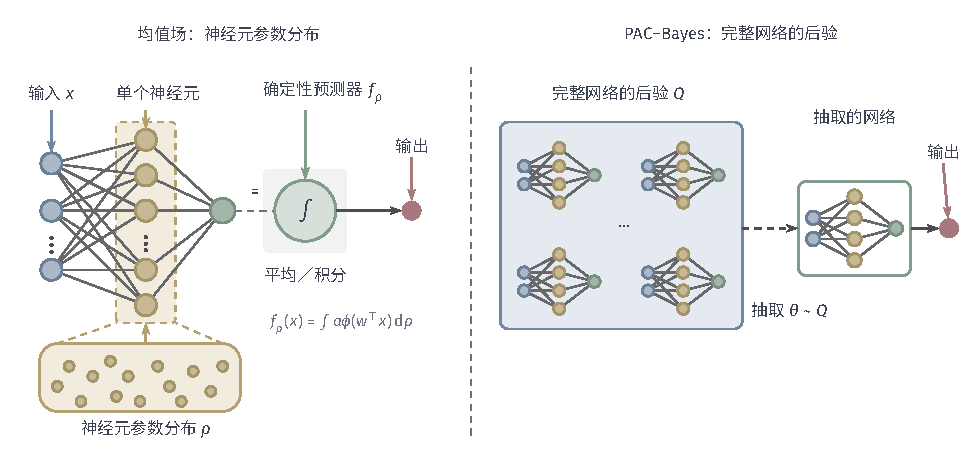
\includegraphics[width=164.600mm]{figures/03-foundations/02-learning-theory/tikz/parameter-distribution-semantics/figure.pdf}
  \caption{两种分布的基本元素不同。平均场侧对单个神经元的贡献$a\phi(\bm w^\top\bm x)$积分，由神经元参数分布$\rho$得到确定性预测器$f_\rho$；神经网络、参数集合与积分表示同一预测器的不同表述，不是对完整神经网络的输出再做集成。PAC--Bayes侧的$Q$以完整参数向量为元素，抽取$\bm\theta$后才得到完整预测器$f_{\bm\theta}$。}
  \label{fig:parameter-distribution-semantics}
\end{figure*}

沿用稳定性思路时，我们要比较只差一个样本的两份训练集分别得到的两个分布有多接近。为什么不直接逐个比较两次训练的参数？因为神经元没有固定编号：训练后单元的顺序可能完全打乱，逐个位置比较参数会把“只是单元顺序不同”的同一神经网络误判为变化很大。Wasserstein距离允许先把两个群体中的单元重新配对，再计算配对后参数的平均距离，因而衡量的是“群体整体挪动了多少”。它可以直观理解为：把一个分布看作一堆土，把另一个分布看作要堆成的形状，距离等于把前者搬成后者所需的最小平均搬运量。写成公式，一阶Wasserstein距离为$W_1(\mu,\nu)=\inf_{\pi\in\Pi(\mu,\nu)}\mathbb E_{(\bm\vartheta,\bm\vartheta')\sim\pi}\|\bm\vartheta-\bm\vartheta'\|_2$，其中$\Pi(\mu,\nu)$是边缘分别为$\mu$和$\nu$的全部联合分布，每个联合分布就是一种搬运（配对）方案。例如一维上，把位于0的全部质量搬到1，距离为1；若只有一半质量需要从0搬到1、另一半不动，距离为0.5。在完备可分度量空间及有限一阶矩条件下，这个距离有限；当前参数空间为欧氏空间，分布均有有限一阶矩。$W_1(\rho_S,\rho_{S'})$在单个神经元的参数空间中比较两个群体，$W_1(Q_S,Q_{S'})$在完整参数空间中比较两个随机神经网络，二者的底层空间不同。

明确了用什么衡量分布接近之后，风险分析还随随机单位改变。神经元分布先经积分变为一个预测函数，再由复杂度或样本稳定性控制泛化；完整神经网络的后验则可与一个独立于样本的先验比较，用相对熵给出随机预测器的风险界。下面分别推导，并说明Wasserstein距离、相对熵和互信息各自比较的是哪两个分布。

\subsection{平均场表示与Wasserstein稳定性接口}

当神经元的特征随训练持续改变时，固定特征的核方法不再适用，逐个记录每个神经元的轨迹又太繁琐。平均场方法的思路是不再区分“第$j$个单元”，而用参数空间中的质量分布描述整个神经元群体：相同参数的单元占多少质量，训练后质量整体怎样移动。先写出这种描述。

取$m$隐藏单元的两层神经网络。为使宽度增加时输出不发散，对每个单元的贡献乘$1/m$缩放：
\[
 f_m(\bm x)=\frac1m\sum_{j=1}^m a_j\phi(\bm w_j^\top\bm x).
\]
给每个$(a_j,\bm w_j)$赋质量$1/m$，得到$\rho_m=m^{-1}\sum_{j=1}^m\delta_{(a_j,\bm w_j)}$，其中$\delta_{(a,\bm w)}$是在$(a,\bm w)$处的点质量分布。求和便等于
\begin{equation}
 f_{\rho_m}(\bm x)=\int a\phi(\bm w^\top\bm x)\,\mathrm d\rho_m(a,\bm w).
 \label{eq:mean-field-network}
\end{equation}
例如四个隐藏单元中，两个取参数$(a,\bm w)=(1,\bm w_1)$，两个取$(-1,\bm w_2)$，则$\rho_4$在这两点上各有质量$1/2$，输出为$\tfrac12\phi(\bm w_1^\top\bm x)-\tfrac12\phi(\bm w_2^\top\bm x)$。把每个单元复制成一百份，宽度变为400，分布和输出都不变。$1/m$缩放正是为了让宽度改变时输出保持在同一尺度上。分布在此表示单个神经网络的组成。与第~\ref{sec:neural-tangent-kernel}节的$1/\sqrt m$缩放对照：那里$m$个单元分摊一次输出改变，每个参数只需移动约$1/\sqrt m$；这里每个单元的贡献已被压到$1/m$，要让输出改变常数量级，各单元参数本身就要移动常数量级，特征因而随训练真正改变。

\term{平均场理论}（mean-field theory）分析适当缩放下，$\rho_m$在宽度$m\to\infty$时趋近连续分布$\rho$后的训练过程。Mei等给出了两层神经网络的这一极限及有限宽近似\scite{mei2018meanfield,mei2019meanfield}。训练中质量会在参数空间中移动，从而改变$\bm w$及其对应的特征，这一点与固定核的惰性训练根本不同。惰性训练与平均场是两种不同的无限宽极限，各自依赖参数随宽度的缩放方式与训练条件，不能简单按“宽神经网络”和“窄神经网络”来划分：同一宽度下，换一种初始化缩放，就可能从一种极限转到另一种。

积分对$\rho$是线性的，所以当预测损失是凸函数时，风险作为分布$\rho$的函数也是凸的。这看起来是个好消息：非凸的神经网络训练似乎变成了一个凸优化问题。但要注意，$\rho$是连续分布，而真实的有限宽神经网络只能移动有限个离散的质量点；我们无法直接对一个连续分布做梯度下降，在有限质量点上优化仍然可能是非凸的。因此分布上的凸性只说明“如果能在整个分布空间中优化”问题会变简单，它没有直接保证普通梯度下降在有限神经网络上能找到全局最优，也没有单独控制样本泛化。

我们进一步比较只替换一个训练样本后得到的两个神经元分布$\rho_S,\rho_{S'}$。直觉上，若替换一个样本只让神经元群体整体挪动一点，积分后的输出就只改变一点，泛化差也就小。为把这一直觉写成可验证的条件，固定参数域$\Theta\subseteq\mathbb R^q$和输入域$\mathcal X$，并假设：神经元输出$\psi_{\bm\vartheta}(\bm x)$对参数一致地为$L_\psi$-Lipschitz（即参数挪动单位距离，任何输入上的单元输出至多改变$L_\psi$），预测损失为$G$-Lipschitz。若相邻样本训练出的分布满足$W_1(\rho_S,\rho_{S'})\leq a_n$，则
\[
 \left|\mathbb E_S\bigl[R(f_{\rho_S})-\hat R_S(f_{\rho_S})\bigr]\right|
 \leq G L_\psi a_n.
\]
这个界的来源可以分两步看清。先看输出差：对任意一种把两个群体中的神经元配对的方式$\pi$（即一个耦合），每对神经元的输出差至多为$L_\psi$乘以参数距离，于是
\[
 |f_{\rho_S}(\bm x)-f_{\rho_{S'}}(\bm x)|
 \leq L_\psi\mathbb E_\pi\|\bm\vartheta-\bm\vartheta'\|_2.
\]
在所有配对中取平均搬运距离最小的那个，就得到$L_\psi W_1(\rho_S,\rho_{S'})$；再乘上损失的Lipschitz常数$G$，并用前一章的替换样本恒等式，便得到泛化差。对$\psi_{(a,\bm w)}(\bm x)=a\phi(\bm w^\top\bm x)$，只要输入、$a$、$\bm w$有界且激活是Lipschitz的，就能验证统一的$L_\psi$存在；换成其他单元形式，只要同样的一致Lipschitz条件成立，界依然有效。

上面的推导只建立了从“分布稳定”到“泛化差小”的接口：若已知$a_n$小，泛化差就小。但它没有从任何具体的训练动力学证明$a_n$确实小——后者还需分析初始化如何耦合、训练多长、损失和势函数的光滑性等。要进一步比较“算法输出与该空间中最优分布的差距”，再固定一个允许的分布集合$\mathcal M$，要求训练输出$\rho_S\in\mathcal M$且它的经验风险与$\mathcal M$中最优经验风险之差满足
\[
 \mathbb E_S\left[
   \hat R_S(f_{\rho_S})
   -\inf_{\rho\in\mathcal M}\hat R_S(f_\rho)
 \right]\leq\xi_n.
\]
这里的$\xi_n$就是第~\ref{sec:deep-general-learning}节风险分解里的经验优化误差$\rho_n$在分布情形下的对应物。把它与泛化差合并（固定$\rho$时经验风险的期望等于总体风险），得到
\begin{equation}
 0\leq
 \mathbb E_S R(f_{\rho_S})
 -\inf_{\rho\in\mathcal M}R(f_\rho)
 \leq G L_\psi a_n+\xi_n.
 \label{eq:mean-field-excess-risk}
\end{equation}
当$a_n\to0$且$\xi_n\to0$时，算法输出的平均期望风险就趋于$\mathcal M$中的最优值。由于左边非负，再用Markov不等式可以把平均结论转成高概率结论：
\[
 \mathbb P\left\{
 R(f_{\rho_S})-\inf_{\rho\in\mathcal M}R(f_\rho)>\varepsilon
 \right\}
 \leq\frac{G L_\psi a_n+\xi_n}{\varepsilon}.
\]
右侧不超过$\delta$时，便得到相应的PAC保证。这也再次印证了第~\ref{sec:deep-general-learning}节的区分：平均界与高概率界是两类结论，转换需要额外付出失败概率的代价。

最终若使用有限宽$f_{\rho_{m,S}}$，还须把逼近$\rho_S$造成的训练及总体风险误差加入式~\eqref{eq:mean-field-excess-risk}。无限神经元极限中的分布收敛，不能单独提供有限宽预测保证。

现在把随机单位从“一个神经网络内的神经元”换成“完整的神经网络”。$\rho$抽出的只是一个单元，还需积分才形成预测；下面的$Q$抽取一次就得到完整的预测器。评价对象变了，风险和参照分布也要重新定义。

\subsection{完整神经网络分布与随机预测器泛化}
\label{sec:pac-bayes}

设算法根据样本$S$在完整参数空间上得到一个分布$Q_S$，预测时先从$Q_S$抽取一组参数，再用这个神经网络预测。注意这里与平均场的区别：平均场是对一个神经网络内部的神经元积分，得到的仍是确定输出；这里是在多个完整神经网络之间随机抽取，每次得到的可能是不同的神经网络。分析这样的随机预测器，按参照对象的不同有三条路线：PAC--Bayes把$Q_S$与一个独立于样本的先验$P_0$比较，给出“对这次抽到的训练集以高概率成立”的界；分布稳定性把$Q_S$与相邻样本产生的$Q_{S'}$比较，给出“对训练集取平均”的泛化差；对相对熵取平均还能联系到算法输出与样本之间的互信息。第~\ref{sec:deep-general-learning}节区分了高概率风险、样本平均风险和经验优化收敛。这里的互信息是控制平均泛化差的工具，不是与高概率、平均并列的第三种概率形式；它与PAC--Bayes及分布稳定性应按参照对象和结论形式分别理解。

\paragraph{PAC--Bayes风险界}

设训练得到的中心参数经验风险很低，而且把它稍加扰动后得到的神经网络损失也都很低。这时与其只评价一个参数点，不如评价中心附近的一整族神经网络：用一个依赖样本的分布描述这一族，同时计算这族随机神经网络的经验风险，以及这个分布相对于事先选定的分布偏离了多少。后者可以理解为“看过数据后改变主意的代价”：训练前就认为很可能的参数，选中它们几乎不需要付出代价；训练前认为不太可能的参数，选中它们就要付出较大代价。这正是PAC--Bayes的比较方式。与范数路线相比，变化在于复杂度不再按最坏方向的放大倍数计算：若训练结果在许多方向上都能承受较大扰动，后验就可以在这些方向上铺得较宽，从而更接近先验、代价更低。

\begin{definition}[PAC--Bayes的先验与后验]
\label{def:pac-bayes-distributions}
设$\Theta$为完整神经网络的参数空间。先验$P_0$是与样本$S$独立的$\Theta$上概率分布，
后验$Q_S$是由$S$决定的$\Theta$上概率分布。对于任意分布$Q$，定义
\[
 \hat R_S(Q)=\mathbb E_{\bm\theta\sim Q}\hat R_S(\bm\theta),
 \qquad R(Q)=\mathbb E_{\bm\theta\sim Q}R(\bm\theta).
\]
\end{definition}

“后验”在此只表示依赖数据的分布，不要求按贝叶斯公式求出。评价时先从$Q$抽取参数再预测，其风险通常不等于“用平均参数构成的那个神经网络”的风险。看一个教学例子：两个候选神经网络的经验错误率分别为0.02和0.10，后验赋予它们概率0.9和0.1，随机预测器的经验错误率为$0.9\times0.02+0.1\times0.10=0.028$。信息代价用相对熵衡量，离散情形下为$D_{\mathrm{KL}}(Q\|P_0)=\sum_kQ(k)\log\bigl(Q(k)/P_0(k)\bigr)$：后验在先验认为不太可能的候选上放的概率越多，这一项越大。若先验对两者各赋$1/2$，信息代价为$D_{\mathrm{KL}}(Q\|P_0)=0.9\log1.8+0.1\log0.2\approx0.368$。若后验把全部概率都给第一个神经网络，经验错误率降到0.02，信息代价却升到$\log2\approx0.693$。经验风险评价预测，相对熵评价概率质量重新分配了多少，PAC--Bayes界在两者之间权衡。

PAC--Bayes界要比较后验的经验风险$\hat R_S(Q)$与总体风险$R(Q)$这两个$[0,1]$中的数。把它们分别看作两枚硬币正面朝上的概率，用两个Bernoulli分布之间的相对熵衡量它们的差距，就得到Bernoulli相对熵
\[
 \operatorname{kl}(a\|b)=a\log\frac ab+(1-a)\log\frac{1-a}{1-b},
\]
端点取连续延拓。它是两个Bernoulli分布的KL散度，一般不对称，不是度量。当$b\in(0,1)$固定且$a$接近$b$时，二阶项为$(a-b)^2/[2b(1-b)]$。保留kl形式可以直接反解风险允许区间；若进一步使用$\operatorname{kl}(a\|b)\geq2(a-b)^2$，会得到较易计算的平方根界，但也丢失关于两概率位置的部分信息。这里比较的是风险界的表达与反解方式，而不是说散度本身比平方差的数值更小。下面使用便于完整推导的常数，不追求最优常数。

\begin{theorem}[PAC--Bayes期望风险界]
\label{thm:pac-bayes-bound}
设$(Z,\mathcal Z)$为可测观测空间，$\mathcal P$为其上的概率分布，
$(\Theta,\mathcal T)$为参数空间。对每个$\bm\theta\in\Theta$，令
$z\mapsto\ell(\bm\theta,z)$为可测的$[0,1]$值损失，并假设联合映射
$(\bm\theta,z)\mapsto\ell(\bm\theta,z)$可测。令
$S=(z_1,\ldots,z_n)\sim\mathcal P^n$，其中$n\geq1$，并定义
\[
 \hat R_S(\bm\theta)=\frac1n\sum_{i=1}^n\ell(\bm\theta,z_i),
 \qquad
 R(\bm\theta)=\mathbb E_{z\sim\mathcal P}\ell(\bm\theta,z).
\]
对$\Theta$上的任意概率分布$Q$，定义
\[
 \hat R_S(Q)=\mathbb E_{\bm\theta\sim Q}\hat R_S(\bm\theta),
 \qquad
 R(Q)=\mathbb E_{\bm\theta\sim Q}R(\bm\theta).
\]
对$a,b\in[0,1]$，定义
\[
 \operatorname{kl}(a\|b)
 =a\log\frac ab+(1-a)\log\frac{1-a}{1-b},
\]
端点按连续延拓解释。
设先验$P_0$为与$S$独立的$\Theta$上概率分布。
对于任意$\delta\in(0,1)$，以至少$1-\delta$的概率，所有$Q\ll P_0$同时满足
\begin{equation}
 \operatorname{kl}\bigl(\hat R_S(Q)\|R(Q)\bigr)
 \leq\frac{D_{\mathrm{KL}}(Q\|P_0)+\log((n+1)/\delta)}{n}.
 \label{eq:pac-bayes-kl}
\end{equation}
从而在同一事件上，
\[
 R(Q)\leq\hat R_S(Q)+
 \sqrt{\frac{D_{\mathrm{KL}}(Q\|P_0)+\log((n+1)/\delta)}{2n}}.
\]
\end{theorem}
证明要解决的难点是：后验$Q$依赖样本，不能直接对它使用只适用于固定参数的集中不等式。办法分三步。先对每个固定参数控制经验风险偏离总体风险的指数矩；再对与样本无关的先验求平均，用Markov不等式得到一个只由样本决定的高概率事件；最后在这个事件上，用换测度不等式把先验下的平均换成任意后验下的平均，换的代价正是相对熵。由于高概率事件不依赖$Q$，结论对所有后验同时成立，后验也就可以在看过样本后再选。
\begin{proof}
固定参数$\bm\theta$，记其期望风险为$r$。
若$r=0$或$r=1$，有界损失几乎处处为相应常量，经验风险也等于$r$，故下面的指数矩等于1，所需上界成立。以下只需考虑$0<r<1$。若单样本损失为Bernoulli变量，经验风险为$k/n$的概率是
$\binom nk r^k(1-r)^{n-k}$，故
\[
 \begin{aligned}
 &\mathbb E_S e^{n\operatorname{kl}(\hat R_S(\bm\theta)\|r)}\\
 &\quad=\sum_{k=0}^n\binom nk
       \left(\frac kn\right)^k\left(1-\frac kn\right)^{n-k}
 \leq n+1.
 \end{aligned}
\]
每一项都是某个二项分布取值于$k$的概率，因而不超过1。
对一般$[0,1]$损失，可依次对每个损失变量条件化。固定其余变量后，所用指数矩关于当前取值是凸函数；取值在$[0,1]$内的变量，按其条件均值换成只取0和1的Bernoulli端点变量，会使该凸函数的条件期望不减小。逐坐标重复这一步，便把一般有界损失的指数矩上界化为前面的Bernoulli情形，因此上界仍然成立。

对独立先验积分，再使用Markov不等式，以至少$1-\delta$的概率有
\[
 \mathbb E_{\bm\theta\sim P_0}
 e^{n\operatorname{kl}(\hat R_S(\bm\theta)\|R(\bm\theta))}
 \leq\frac{n+1}{\delta}.
\]
在这个只由样本决定的事件上，对任意$Q\ll P_0$使用换测度不等式
\begin{equation}
 \mathbb E_Q g\leq D_{\mathrm{KL}}(Q\|P_0)+\log\mathbb E_{P_0}e^g,
 \label{eq:change-of-measure}
\end{equation}
其推导见式~\eqref{eq:information-change-measure}。
取$g(\bm\theta)=n\operatorname{kl}(\hat R_S(\bm\theta)\|R(\bm\theta))$，
再由$\operatorname{kl}$的联合凸性把左侧下界为
$n\operatorname{kl}(\hat R_S(Q)\|R(Q))$，即得第一式。
最后使用$\operatorname{kl}(a\|b)\geq2(a-b)^2$得到第二式。
\end{proof}

Maurer的精细指数矩估计可在相应条件下把$n+1$换成$2\sqrt n$\scite{maurer2004pacbayes}。风险界还需小后验经验风险才有低总体风险；相对于假设空间的PAC学习则须进一步证明算法找到经验误差小且相对熵增长足够慢的后验。

若后验满足$D_{\mathrm{KL}}(Q_S\|P_0)\leq K$，我们可直接要求
\begin{equation}
 2n\varepsilon^2\geq K+\log((n+1)/\delta)
 \label{eq:pac-bayes-sample-requirement}
\end{equation}
使经验风险外的代价不超过$\varepsilon$。忽略$n$的对数，充分样本量随$(K+\log(1/\delta))/\varepsilon^2$增长。作为教学读界例子，经验风险至多0.02、附加量至多0.03，便以概率至少$1-\delta$得到随机预测风险至多0.05；这些数值不代表实测结果。

如果整个后验的平均经验风险为零，可直接利用$\operatorname{kl}(0\|r)=-\log(1-r)$，在同一事件中得到
\[
 R(Q_S)\leq1-\exp\left(-\frac{K+\log((n+1)/\delta)}n\right)
 \leq\frac{K+\log((n+1)/\delta)}n.
\]
此时充分条件为$n\varepsilon\geq K+\log((n+1)/\delta)$。中心神经网络分类正确尚不足以使后验平均经验风险为零，因此不能据此直接使用该速率。

PAC--Bayes用相对于独立先验的代价$K$衡量复杂度，而不是数参数，所以参数很多的神经网络也可能代价很小；但这个代价必须对具体后验实际算出来，不能凭参数个数估计。构造后验时，扰动后的经验损失与信息代价需要共同控制：把后验铺得更宽可以让它更接近先验、降低信息代价，却可能覆盖到损失较高的参数；把后验收窄到训练中心附近可以保持低损失，信息代价却会上升。下面以高斯分布说明这个取舍。

连续先验下，若后验把全部质量放在单个训练参数上，相对熵通常为无穷大，界没有意义。因此改取$Q=\mathcal N(\hat{\bm\theta},\sigma^2\bm I)$，把中心附近的完整神经网络都纳入评价。对$p$维先验$P_0=\mathcal N(0,\tau^2\bm I)$，有
\begin{equation}
 D_{\mathrm{KL}}(Q\|P_0)=\frac{\|\hat{\bm\theta}\|_2^2}{2\tau^2}
 +\frac p2\left(\frac{\sigma^2}{\tau^2}-1-\log\frac{\sigma^2}{\tau^2}\right).
 \label{eq:gaussian-pac-bayes-kl}
\end{equation}
它由两个各向同性高斯分布的相对熵公式得到：均值差贡献$\|\hat{\bm\theta}\|_2^2/(2\tau^2)$，每个坐标的方差不一致再各贡献$\tfrac12(\sigma^2/\tau^2-1-\log(\sigma^2/\tau^2))$，共$p$个坐标。式中第一项是中心离先验均值有多远，第二项是后验宽度与先验宽度不一致的代价。第二项乘着参数维数$p$，在大型神经网络中可能很大。例如$p=10^6$、$\sigma^2=\tau^2/2$时，第二项为$\tfrac{10^6}2(\tfrac12-1-\log\tfrac12)\approx9.7\times10^4$；若样本数只有$10^5$，界中的$\sqrt{K/(2n)}$就接近0.7，几乎没有信息。只有后验宽度与先验接近、或者只在少数方向上收窄，这一项才会小。

当损失较低的区域较大时，可以扩大后验以覆盖更多低损失神经网络，但方差代价在$\sigma^2=\tau^2$处最小，向两侧偏离都会增大。因此，所谓解的平坦性（即损失在最优点附近是平缓的宽谷还是陡峭的窄谷）必须落实为“扰动后损失增加多少”与“相对熵代价”的比较；单看Hessian或谷宽仍受参数化影响\scite{dinh2017sharp}。

图~\ref{fig:learning-flat-sharp}固定坐标、方向和参数化，对比同等扰动的经验风险增幅。宽谷在此方向上增幅较小，说明局部扰动代价较低，尚需后验经验风险与先验代价共同支持泛化。重缩放坐标可以改变谷宽，所以截面宽窄不是函数本身不变的风险属性。

\begin{figure*}[htbp]
  \centering
  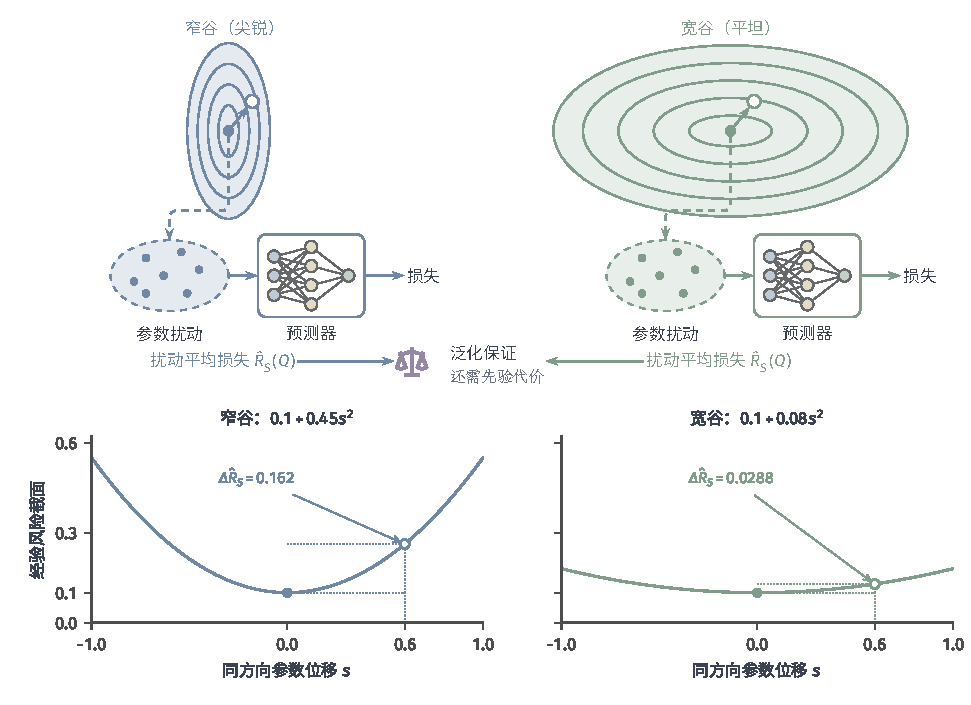
\includegraphics[width=164.600mm]{figures/03-foundations/02-learning-theory/tikz/learning-theory-flat-sharp/figure.pdf}
  \caption{参数扰动代价与PAC--Bayes中的两项控制。上部示意窄谷、宽谷附近的参数扰动与随机预测器；在相应定理条件下，泛化保证还需同时控制后验经验风险与相对于独立先验的相对熵代价。下部两个面板共用相同横纵尺度，横轴为同一单位方向上的参数位移$s$，即$\bm\theta=\hat{\bm\theta}+s\bm u$、$\|\bm u\|_2=1$。构造的窄谷与宽谷分别为$0.1+0.45s^2$、$0.1+0.08s^2$；实心点为谷底，空心点对应相同位移$s=0.6$，经验风险分别增加0.162和0.0288。上部轮廓没有数值含义，下部曲线仅为可复算的教学构造。谷的宽度受参数化与坐标尺度影响，宽谷不必具有较小的期望风险。}
 \label{fig:learning-flat-sharp}
\end{figure*}

\paragraph{后验分布的稳定性}

现在换一个参照对象：PAC--Bayes比较$Q_S$与固定的先验$P_0$，稳定性则比较$Q_S$与相邻样本产生的$Q_{S'}$。两种比较互不蕴含：后验离先验很近，并不意味着替换一个样本后后验几乎不变；反之亦然。

稳定性路线的思路与前面相同。若能把两个后验中的神经网络两两配对，使配对的参数平均相距很近，而损失关于完整参数是Lipschitz的，那么两个随机预测器的平均损失就相差很小。下面把这个配对距离，即Wasserstein距离，直接接到泛化恒等式。

\begin{theorem}[参数分布稳定性与期望泛化差]
\label{thm:distribution-stability-generalization}
设$(Z,\mathcal Z)$为可测观测空间，$\mathcal P$为其上的概率分布，
$S=(z_1,\ldots,z_n)\sim\mathcal P^n$，其中$n\geq1$。
参数空间$\Omega\subseteq\mathbb R^p$取Borel $\sigma$代数；可测随机学习算法根据
$S$输出具有有限一阶矩的概率分布$Q_S$，再抽取$\bm\theta\sim Q_S$。
设损失$\ell:\Omega\times Z\to[0,1]$联合可测，并且对每个$z\in Z$及任意
$\bm\theta,\bm\theta'\in\Omega$都有
\[
 |\ell(\bm\theta,z)-\ell(\bm\theta',z)|
 \leq L_\theta\|\bm\theta-\bm\theta'\|_2.
\]
定义
\[
 \begin{aligned}
 R(\bm\theta)&=\mathbb E_{z\sim\mathcal P}\ell(\bm\theta,z),&
 \hat R_S(\bm\theta)&=\frac1n\sum_{i=1}^n\ell(\bm\theta,z_i),\\
 R(Q)&=\mathbb E_{\bm\theta\sim Q}R(\bm\theta),&
 \hat R_S(Q)&=\mathbb E_{\bm\theta\sim Q}\hat R_S(\bm\theta).
 \end{aligned}
\]
其中$L_\theta,\alpha_n\geq0$。若任意仅替换一条观测所得的相邻样本$S,S'$都满足
$W_1(Q_S,Q_{S'})\leq\alpha_n$，则
\[
 \begin{aligned}
 \sup_z\left|\mathbb E_{Q_S}\ell(\bm\theta,z)
              -\mathbb E_{Q_{S'}}\ell(\bm\theta,z)\right|
 &\leq L_\theta\alpha_n,\\
 \left|\mathbb E_S[R(Q_S)-\hat R_S(Q_S)]\right|
 &\leq L_\theta\alpha_n.
 \end{aligned}
\]
进一步，若$\Theta\subseteq\Omega$为可测比较决策空间、$\rho_n\geq0$、
$Q_S(\Theta)=1$几乎必然成立，且
\[
 \mathbb E_S\left[\hat R_S(Q_S)-\inf_{\bm\theta\in\Theta}
                           \hat R_S(\bm\theta)\right]\leq\rho_n,
\]
则$\mathbb E_S R(Q_S)-\inf_{\bm\theta\in\Theta}R(\bm\theta)
\leq L_\theta\alpha_n+\rho_n$。
若这两个速率对所有允许分布一致趋于零，则得到相对于$\Theta$的随机PAC学习保证。
\end{theorem}
\begin{proof}
对任意配对分布$\pi\in\Pi(Q_S,Q_{S'})$，损失期望之差的绝对值不超过
\[
 \mathbb E_\pi|\ell(\bm\theta,z)-\ell(\bm\theta',z)|
 \leq L_\theta\mathbb E_\pi\|\bm\theta-\bm\theta'\|_2.
\]
对$\pi$取下确界得到均匀稳定性，再由前章的替换样本恒等式得到期望泛化差。
对于任意固定$\bm\theta\in\Theta$，近似ERM条件给出
$\mathbb E_S\hat R_S(Q_S)\leq R(\bm\theta)+\rho_n$。
加上泛化差并取下确界即得超额期望风险界。
由于$Q_S$以$\Theta$为支撑，联合随机变量
$R(\bm\theta)-\inf_{\bm\vartheta\in\Theta}R(\bm\vartheta)$非负，且
\[
 \mathbb E_{S,\,\bm\theta\sim Q_S}
 \left[R(\bm\theta)-\inf_{\bm\vartheta\in\Theta}R(\bm\vartheta)\right]
 =\mathbb E_S R(Q_S)-\inf_{\bm\vartheta\in\Theta}R(\bm\vartheta)
 \leq L_\theta\alpha_n+\rho_n.
\]
对这个联合随机变量应用Markov不等式，失败概率至多
$(L_\theta\alpha_n+\rho_n)/\varepsilon$；令它不超过$\delta$即得到同时包含样本和
后验抽样随机性的PAC保证。
\end{proof}

已有$W_1(Q_S,Q_{S'})\leq c/n$和$\rho_n\leq c'/\sqrt n$时，稳定性与经验最优性给出
\[
 \mathbb E_S R(Q_S)-\inf_{\bm\theta\in\Theta}R(\bm\theta)
 \leq\frac{L_\theta c}{n}+\frac{c'}{\sqrt n}.
\]
例如$n\geq\max\{2L_\theta c/\varepsilon,\,4(c')^2/\varepsilon^2\}$足以使平均超额风险不超过$\varepsilon$。这是对给定速率的条件推论，具体神经网络仍需训练分析来证明这些速率。

参数耦合难以估计时，还可比较相邻后验总变差。$[0,1]$损失的期望差不超过该距离，再由$\sqrt{D_{\mathrm{KL}}(Q_S\|Q_{S'})/2}$控制。此处相对熵两端都是相邻后验，不能直接替换为后验—先验代价。

\paragraph{相对熵与互信息}

若随机输出为$W$、边缘分布为$\bar Q=\mathbb E_SQ_S$，相关相对熵有限时有
\begin{equation}
 \mathbb E_SD_{\mathrm{KL}}(Q_S\|P_0)
 =I(W;S)+D_{\mathrm{KL}}(\bar Q\|P_0).
 \label{eq:pac-bayes-information-decomposition}
\end{equation}
将对数密度比分成$\log(\mathrm dQ_S/\mathrm d\bar Q)$和$\log(\mathrm d\bar Q/\mathrm dP_0)$再平均，即得此式。两项含义不同。第一项是互信息，衡量输出$W$平均从这一份具体样本中获取了多少信息：若不论样本如何，算法给出的后验都差不多，这一项就很小。第二项衡量所有样本平均下来的输出分布与先验差多远，与具体样本无关；若先验恰好取为平均输出分布$\bar Q$，第二项为零。这个分解联系了平均的PAC--Bayes代价与信息稳定性，但并没有把互信息给出的期望保证变成对每份样本都成立的高概率保证。

若平均先验代价满足$\mathbb E_SD_{\mathrm{KL}}(Q_S\|P_0)\leq K_n$，第二项非负给出$I(W;S)\leq K_n$，定理~\ref{thm:mutual-information-risk}便得到
\[
 \left|\mathbb E_S[R(Q_S)-\hat R_S(Q_S)]\right|
 \leq\sqrt{\frac{K_n}{2n}}.
\]
参数分布由此沿一般信息稳定性进入风险分解，再与经验最优性合并。PAC--Bayes另给样本高概率事件中的同时后验保证，两种概率对象仍不同。

\paragraph{两类参数分布的联系与边界}

回到两种随机单位的区别：从$\rho_S$抽取一次只得到一个神经元，要经式~\eqref{eq:mean-field-network}的积分才得到完整的$f_{\rho_S}$；从$Q_S$抽取一次就得到一个完整神经网络。所以前者评价的是一个确定的积分函数的风险，后者的$R(Q_S)$是许多完整函数的风险的平均。

三种距离的用途也随单位而定：$W_1(\rho_S,\rho_{S'})$经单元的Lipschitz性控制积分函数的稳定性；$W_1(Q_S,Q_{S'})$经完整参数的Lipschitz性控制随机输出的稳定性；$D_{\mathrm{KL}}(Q_S\|P_0)$则用于换测度，给出高概率界。其中任何一个小，都不会无条件地使另外两个小。

可以在更高层让算法随机输出神经元分布，再以其完整积分预测器组成PAC--Bayes后验。但要重新定义随机对象、先验与损失，并核对可测性和绝对连续性。这并非平均场极限的直接结果。两条分支是不同的分析方式，而不是一个定理的两种表述。

\FloatBarrier
\section{理论的比较与使用}
\label{sec:deep-theory-comparison}

四个入口都在解释同一件事：有限样本训练为什么可能得到期望风险小的神经网络。它们的分工不同：范数路线约束所得函数的复杂度，初始梯度路线固定特征，更新路线说明训练选了哪个解，分布路线进一步区分神经元群体和随机神经网络。表~\ref{tab:deep-generalization-routes}据此整理它们与一般学习工具的关系。复杂度、稳定性和PAC--Bayes是把这些入口连到风险的工具，不是与之并列、互相排斥的另一组入口。

回到章首的邮件分类器，可以看出四条路线各自要求我们检查什么。按范数路线，要看训练后各层参数矩阵的谱范数和训练样本的分类间隔，代入谱复杂度界；按初始梯度路线，要先确认训练中核几乎不变，再算标签在核特征方向上的分量；按更新路线，要说明所用的初始化和优化器偏向哪类解，并证明这类解的范数或间隔受控；按分布路线，则要构造训练结果附近的后验，计算它的经验风险和信息代价。四种检查需要的信息不同，适用的情形也不同。

这些界目前还不能直接按数值大小排名，因为它们的前提并不一致。范数间隔界评价分类错误率，固定特征界评价有界Lipschitz损失，最小范数回归使用平方损失，PAC--Bayes评价随机预测器；式~\eqref{eq:ntk-pac-bayes-risk}还要额外付出扰动代价才能转回中心神经网络。因此必须先统一损失、输出形式与置信要求，再比较右侧的数值。

\begin{table*}[!htb]
 \centering
 \small
 \begin{tabular}{p{24mm}p{43mm}p{46mm}p{38mm}}
 \toprule
 分析入口 & 与一般学习理论的联系 & 期望风险与样本量由什么控制 & 对训练的指导\\
 \midrule
 参数大小 & 函数空间复杂度控制泛化；分层参数变化也可转为损失稳定性 & 经验间隔错误率、范数与间隔之比、样本量及置信度 & 同时控制范数与经验间隔，不能只缩小参数\\
 参数梯度初始值 & 固定特征接上RKHS复杂度、PAC--Bayes与正则化稳定性 & 标签与核谱的关系、RKHS范数、样本量和近似误差 & 检查初始特征能否以较小范数表达目标\\
 参数梯度更新 & 动力学确定选解，再用风险分解、复杂度或稳定性控制泛化 & 最小范数解的数据依赖风险、归一化间隔、矩阵谱与样本敏感性 & 检查初始化、损失、参数化和优化器怎样共同选择解\\
 参数分布 & 神经元分布通过稳定性分析确定性积分模型；完整神经网络分布通过PAC--Bayes或稳定性分析随机预测器 & 神经元分布变化、有限宽度误差、后验经验风险、相对熵代价与置信度 & 先区分$\rho$与$Q$的随机单位，再选择相应距离和泛化结论\\
 \bottomrule
 \end{tabular}
 \caption{神经网络泛化分析的四个入口。每一行对应本章一个上位分析角度；
 具体的复杂度界、稳定性定理和PAC--Bayes界是连接该角度与期望风险的工具。}
 \label{tab:deep-generalization-routes}
\end{table*}

同一个训练结果可以沿多个入口分析。隐式偏差说明训练选出了低范数的解之后，范数间隔界可以评价它的分类风险，样本稳定性则提供另一种保证。初始特征几乎固定时，可用RKHS范数和正则化分析；特征明显变化时，转向真实动力学或神经元分布。PAC--Bayes也可以评价训练结果附近的神经网络，但它直接评价的仍是相应的随机预测器。

设计训练方案时，应分清各项操作改变了什么。范数约束限制允许选择的参数范围，$\ell_2$惩罚改变优化目标，权重衰减（weight decay）则在更新时直接按比例缩小所选参数。初始化和优化器也会影响训练最终得到哪组参数。PAC--Bayes先验在观察当前样本前固定，可以只用于训练结束后的风险评价，不必参与训练。因此，这些做法虽然都可能影响泛化分析，却不是同一种假设空间限制。

更强的约束还可能排除有用的函数。缩小范数球可以降低复杂度，但若目标函数需要较大的范数才能表示，它就不在球内了，即使达到球内的最优风险，仍会留下近似误差。评价一个训练方案时，我们要分别检查三件事：假设空间是否包含风险低的函数，算法是否达到了低经验风险，以及输出是否满足某条泛化界的条件。现有工具能支持这些判断，但没有给出对任意任务都适用的结构与训练选择方法。

推算样本量时，先固定风险目标和能达到的经验误差，再求使附加项足够小的$n$。若范数、间隔、稳定性或后验代价本身随$n$变化，都要一起代入。固定其他量得到的缩放关系只是条件结论；上界过于宽松时，需要针对具体分布和算法做更细的分析，而且无论如何都不能把上界当作测试错误率。

\FloatBarrier
\Needspace{8\baselineskip}
\section{本章小结}
\label{sec:deep-learning-summary}

本章从一个问题出发：参数远多于样本的神经网络能把训练数据全部拟合，为什么在新样本上仍可能表现良好？第一个回答是否定性的：只看参数个数或VC维无法解释这一点。按整个架构计算的保证所需样本量往往远大于实际样本量；随机标签实验进一步说明，同一个架构既能拟合真实规律，也能记住毫无规律的标签，所以任何只依赖架构和样本量的分布无关保证，在这一样本量下都必然空洞。要解释泛化，必须利用数据分布以及训练实际得到的结果有什么性质。

围绕“结果有什么性质”，本章给出四类回答，后一类补上前一类留下的缺口。范数与间隔用所得参数的数值代替参数计数：若参数范数相对于分类间隔较小，风险界可以与宽度无关，但它假定训练已得到这样的参数。初始梯度回答训练如何拟合、选中哪个函数：在惰性训练条件下，神经网络近似为核模型，风险由标签在核特征方向上的分布决定，代价是特征被冻结。梯度更新去掉这一近似：从零出发的梯度下降偏好最小范数解，逻辑损失的方向趋于最大间隔，深层分解偏好近似低秩的矩阵，但完整证明限于可解模型。参数分布则从神经元群体和随机神经网络两个角度给出稳定性与PAC--Bayes保证，分别处理特征改变的宽神经网络和对扰动不敏感的训练结果。这些性质只有连同训练误差、近似能力和样本量一起分析，才构成学习保证；核正定只保证能够插值，最小范数和最大间隔只在各自条件下成立，平均场与PAC--Bayes也各有前提。

这些路线还可以通过稳定性统一起来：范数限制参数变化被放大的程度，动力学决定替换样本后轨迹相差多少，分布距离和信息量控制随机输出对样本的依赖。需要区分的是，训练中相邻两步接近只说明单步更新变小，不能单凭它判定经验目标已经优化完成。相邻训练集上的输出接近则是稳定性信息，须经Lipschitz或其他损失条件转换，才能控制相应的平均或高概率泛化差。沿稳定性得到学习保证时还必须计入经验优化误差；复杂度与PAC--Bayes则提供另外的充分条件。

所有结论都绑定于明确的模型、数据和训练设定。模型规模、训练时长或任务一起变化时，须重新说明哪些量固定、哪些量变化。下一章进一步改变数据分布、学习目标和历史数据访问方式，研究已有信息如何支持迁移与持续学习中的总体风险保证。

\Needspace{18\baselineskip}
\paragraph{扩展阅读}
Bartlett、Foster与Telgarsky的谱归一化间隔分析展示各层范数和分类间隔怎样共同进入风险。可对照神经网络等价缩放，检查为何单独缩小参数或只报参数数目都不足以评价分类保证\scite{bartlett2017spectral}。

Arora等的两层神经网络分析适合追踪核谱与标签如何同时影响训练和风险；Soudry等的可分分类分析则说明逻辑参数发散时方向为何仍趋向最大间隔\scite{arora2019finegrained,soudry2018implicit}。

Maurer的PAC--Bayes推导可用于核对先验积分、指数矩和换测度步骤，尤其可比较更精细常数需要哪些条件\scite{maurer2004pacbayes}。

Razin与Cohen的矩阵分解反例展示范数解释的边界：训练偏好可能无法由固定矩阵范数完整表示，可结合前面的谱动力学与静态范数引理对照\scite{razin2020norms}。
